\begin{quote}
\textit{``Where are you?'' Hiro says.
\\
\\
``In Reality or the Metaverse?''
\\
\\
``Both.''}
\end{quote}
\hfill \textit{Snow Crash, Neal Stephenson}
\\
\\
\\

%=========================================================================================================
%=========================================================================================================

% 'Position' section from experimental plan document

%\section{Introduction}

The subject of this thesis is the design, development \& evaluation of platforms that allow their users to observe \& move around their real environment whilst also being able to view an alternative virtual environment from the equivalent vantage point. This combination of `parallel' real \& virtual environments, combined with maintained mobility, is not well encapsulated by any previously defined alternate reality terminology, thus it is necessary to explore this alternate reality terminology \& technologies in order to correctly frame these systems in relation to them.

The closest existing label is the \textit{cross reality} paradigm, as a cross reality system holds the distinction of two discrete environments, one real \& one virtual, complete-unto-themselves, however cross reality further focusses on a bidirectional exchange of information between the environments \& not upon user mobility \& tandem visual exploration of both environments.

Thus, we propose the new term \textit{parallel reality} to refer to systems that combine complete \& discrete real \& virtual environments together in a manner that allows mobile exploration of them both in tandem, relating it \& positioning it against existing alternate reality terminology previously explored by computer science \& other disciplines.

%This research centres around the design, development \& evaluation of a hardware \& software platform which allows its user to observe \& move around their Real World (RW) environment whilst wearing a wide field of view (FOV), stereoscopic 3D, Head Mounted Display (HMD) which allows them to alternatively view an immersive Virtual Reality (VR) environment from the equivalent vantage point. This is achieved by combining a head-tracked HMD, webcams, an indoor positioning system (IPS) \& a 3D game engine, into a mobile \textit{cross reality} (XR) interface.

%One of the distinguishing features of XR is that, by linking real \& virtual environments more closely, it mitigates the `vacancy problem': \textit{``the noticeable \& profound absence of a person from one world, either real or virtual, while they are participating in the other''}, which arises \textit{``because people do not currently have the means to be in more than one place (reality) at a time''}~\cite{Lifton2007a}.

%Previous XR research approached the vacancy problem by integrating sensor/actuator networks into the environments, such that actions in one could manifest in the other, however direct visual engagement with the virtual environment was only possible from static interfaces at pre-determined locations within the real environment~\cite{Lifton2007a, Dublon2011}. The platform discussed in this document addresses this shortcoming by providing a mobile interface for visual engagement with both environments of a XR system, allowing the user to transition between viewing their real environment \& a virtual environment at any time while maintaining the freedom to move around them, multiplexing visual stimuli from their real surroundings \& from a parallel, virtual `mirror world'~\cite{Gelernter1993}.

%=========================================================================================================
%=========================================================================================================

\section{Defining Alternate Realities}

Alternate realities have received substantial attention in recent decades, the themes explored for purposes as diverse as education~\cite{Warburton2009} \& new forms of data visualisation~\cite{Coleman2009} to medical~\cite{TenEyck2011} \& military training~\cite{Qiu2009}. Although terms such as \textit{mixed reality} \& \textit{augmented reality} are now relatively common in conversation \& literature, definitions of such terms have often been used in vague \& even conflicting manners.

This chapter will investigate popular definitions, classifications \& comparisons of alternate realities, combining \& modifying these parameters to produce a canonical set of definitions for the remainder of this thesis, explaining `parallel reality' into these definitions \& models.

\subsection{Milgram \& Kishino's Reality-Virtuality Continuum}

Paul Milgram, Herman Colquhon and Fumio Kishino addressed the issue of alternate reality definitions in detail and can be accredited with introducing the terms \textit{augmented virtuality} and \textit{mixed reality} to the literature, prompted by their identification of the need for more encompassing terms to supplement the existing definitions of \textit{augmented reality}~\cite{Milgram1994, Milgram1999}.

%However despite these thorough and well-reasoned definitions being published originally in 1994, much of the subsequent literature studied for this review has adopted conflicting, or at least confusing and misleading, definitions.

One of the overbearing concepts introduced by Milgram et al. is that whilst both purely real and purely virtual environments do exist they should not be considered discrete alternatives but rather poles lying at opposite ends of a linear scale $-$ the \textit{Reality-Virtuality continuum}. The location of an environment along this continuum coincides with its location along a parallel \textit{Extent of World Knowledge continuum} where `world knowledge' refers to the amount of quantitative information that is associated with the content being presented, or in other words how much of the environment is being `modelled' by a computer. These continua are included as figure \ref{reality_virtuality_extent_of_world_knowledge_continuum}.

\begin{figure}[h]
\centering

\includegraphics[width=\textwidth]{virtuality_continuum_extent_of_world_knowledge_continuum.png}
\caption{\textit{Reality-Virtuality continuum} (top), parallel with \textit{Extent of World Knowledge continuum} (bottom).}
\label{reality_virtuality_extent_of_world_knowledge_continuum}
\end{figure}

With a purely virtual environment, the entire viewport must necessarily be computer modelled in order to be rendered and as such there is complete quantitative information about all objects and between all objects being presented. At the opposite end of the spectrum with a completely real environment where none of the viewport is computer modelled there is no quantitative information associated with the content being displayed. At any point between the extremes the environment consists of a mixture of some modelled and some non-modelled content; with the computer associating quantitative information to, and between, the virtual objects, but not to the real objects or between the virtual and real objects.

Carrying the continuum concept further, Milgram et al. illustrate their understanding of the existing term \textit{augmented reality} and also introduce two related new terms; \textit{augmented virtuality} and \textit{mixed reality}. In this fashion, \textit{mixed reality} is used to describe any environment that is not completely real or completely virtual; that is, it encompasses all positions on the continuum between the extremes. \textit{Augmented reality} is used to describe a real environment upon which virtual objects are overlain and \textit{augmented virtuality} is used to describe a virtual environment upon which objects sampled from the real world (such as video feeds) are overlain. It is also shown here that \textit{mixed reality} encompasses both \textit{augmented reality} and \textit{augmented virtuality}.

One obvious question raised from studying this figure is at what point toward the centre of the continuum an environment changes from being \textit{augmented reality} into \textit{augmented virtuality} or vice-versa. The answer lies with consideration of the quantitative knowledge associated with the objects that comprise the viewport.

For example, if one were to take a viewport depicting a purely real environment and then incrementally add more and more virtual objects, the environment's classification would progress rightward along the continuum. Eventually the entire viewport would be obscured by virtual objects and the obvious conclusion would be to classify the environment as being purely virtual. However this would only be true if there was complete quantitative information associated with, and between, all of the virtual objects within the real 3D space of the viewport, which is unlikely to be the case.

Likewise if one were to take a viewport depicting a purely virtual environment and incrementally replace the entire viewport with sampled real objects we could not classify the resultant environment as purely real as there would be associated quantitative knowledge with and between the sampled objects, meaning that the environment isn't completely unmodelled and thus can't be classified as purely real.

Thus, Milgram et al. conclude, it is not necessarily true that an environment is purely virtual simply because all of the visible objects are computer modelled, nor is it necessarily true that an environment is purely real simply because all of the visible objects are sampled from the real world.

%=========================================================================================================

\subsection{Roy Want's Virtuality Matrix}

Another method of illustrating the relationships between different categories of alternate realities was put forward by Roy Want in his introductory article for a 2009 issue of IEEE Pervasive Computing dedicated to the \textit{cross reality} paradigm~\cite{Want2009}. He presents a 2x2 matrix categorising the different terms according to whether the experience and overlay data are real or virtual (figure \ref{original_virtuality_matrix.png}). Whilst this is a useful representation, some of the definitions \& criteria depicted do not match with those of Milgram et al. or even with those of other authors in the same issue of Pervasive, let alone other publications concerning alternate realities. Figure \ref{modified_virtuality_matrix.png} presents a modified version of this matrix that is in keeping with the framework laid out by Milgram et al. \& the wider literature.

\begin{figure}[h]
\centering
\begin{minipage}{.5\textwidth}
 	\centering
 	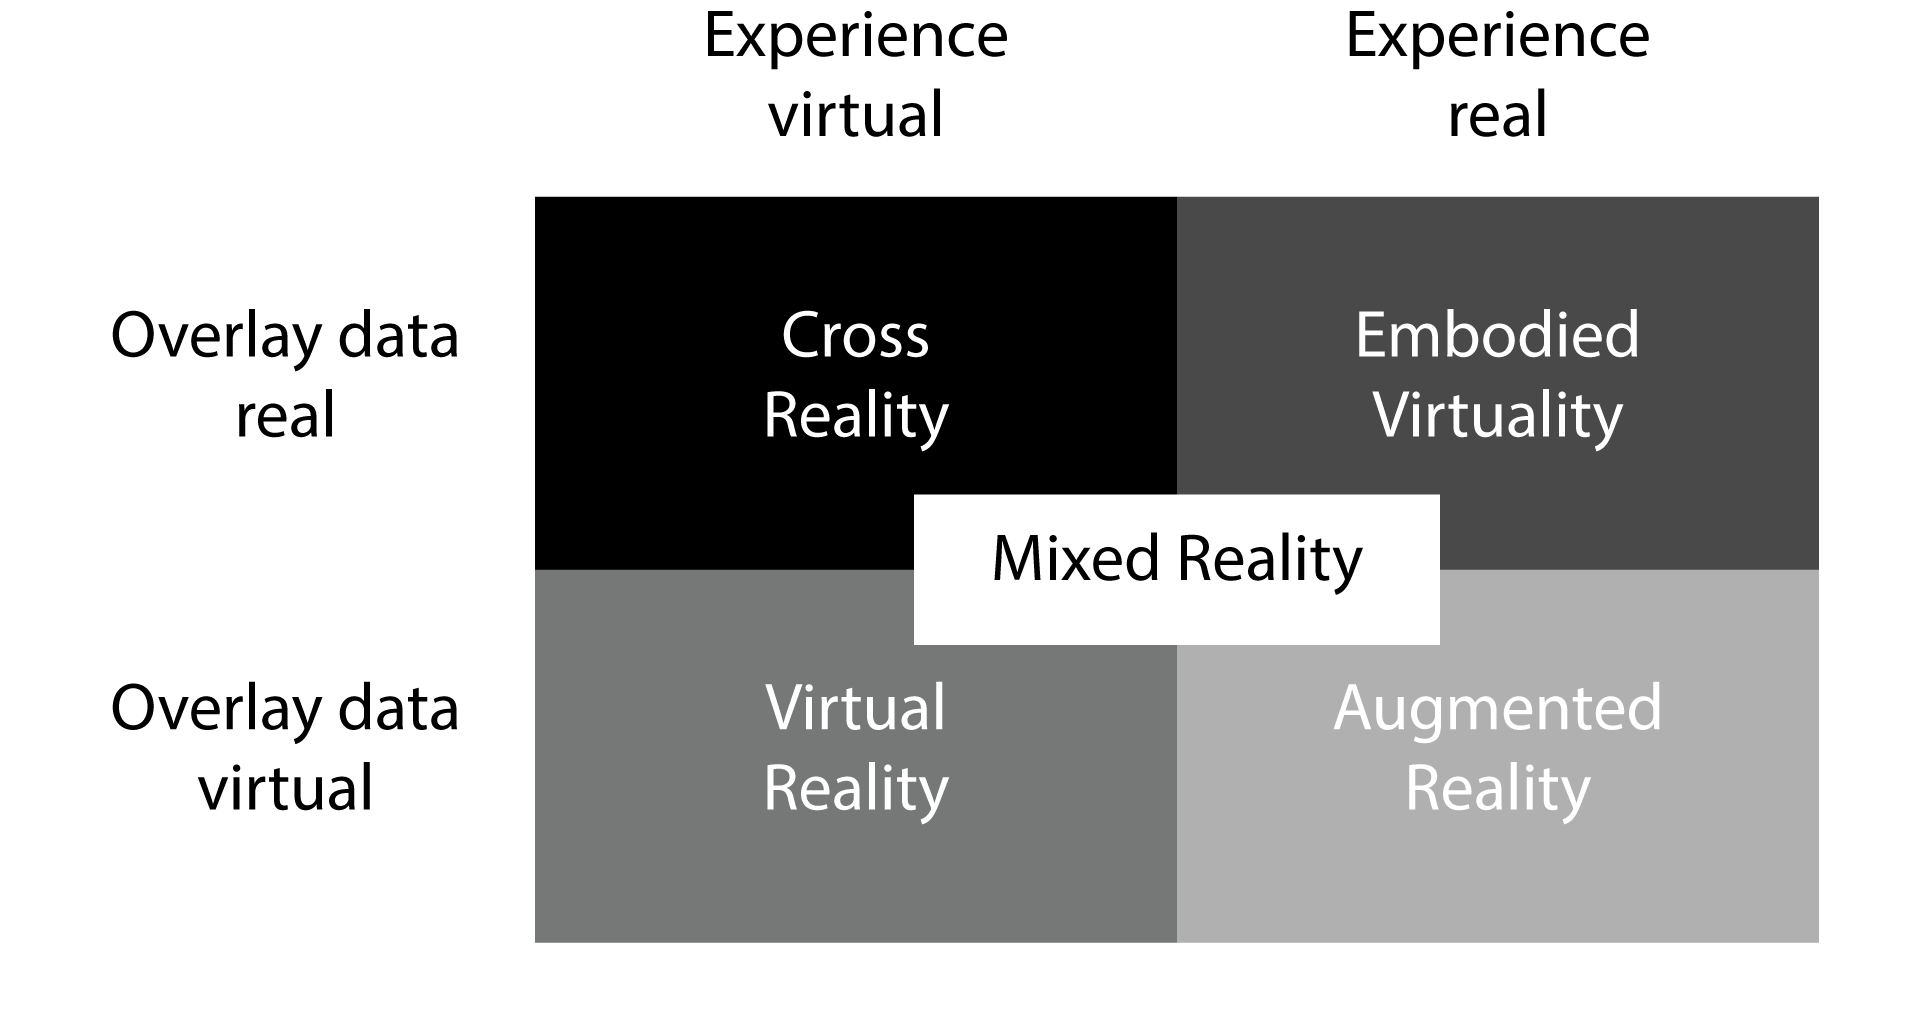
\includegraphics[width=0.95\linewidth]{Want_virtuality_matrix_original.png}
 	\caption{Want's original virtuality matrix.}
	\label{original_virtuality_matrix.png}
\end{minipage}%
\begin{minipage}{.5\textwidth}
  \centering
  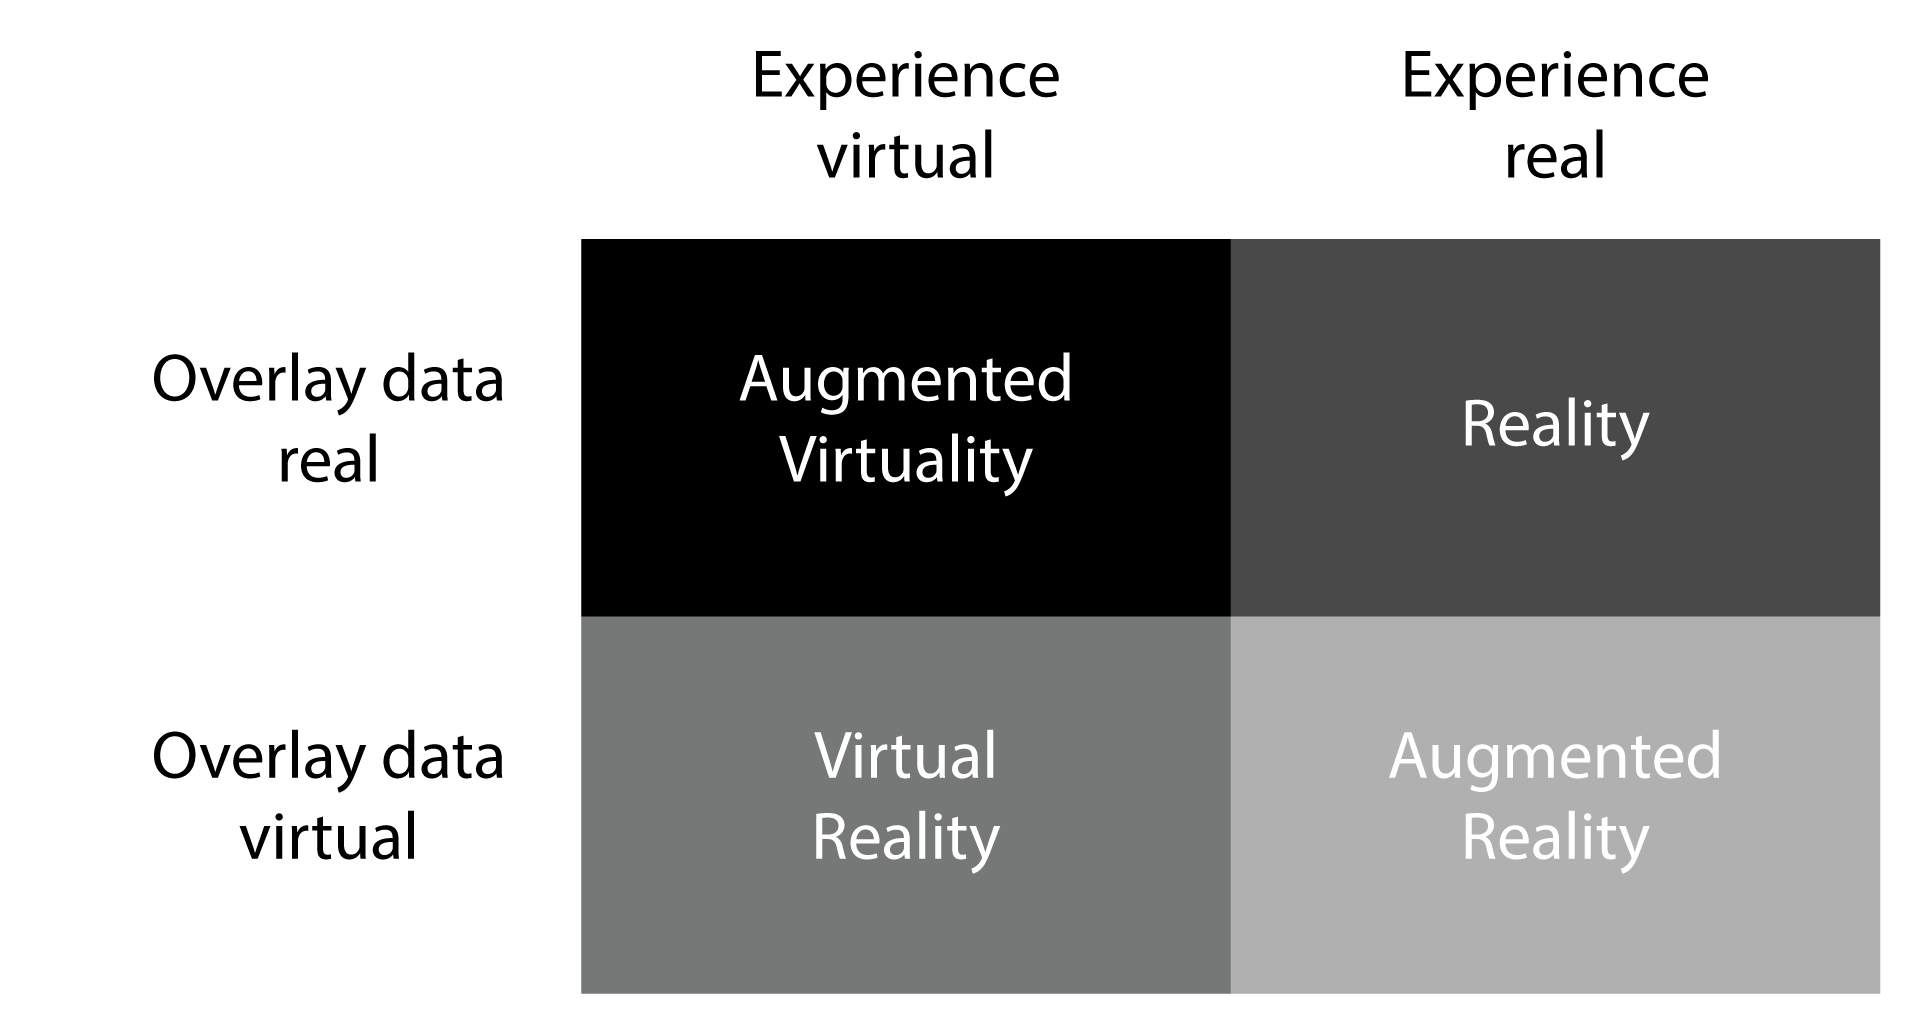
\includegraphics[width=0.95\linewidth]{Want_virtuality_matrix_modified.png}
    \caption{Modified Want matrix.}
    \label{modified_virtuality_matrix.png}
\end{minipage}
\end{figure}

Where the original matrix positions \textit{cross reality} in the upper left quadrant, at the congruence of `experience virtual' and `overlay data real', the modified matrix positions \textit{augmented virtuality}. Referencing Milgram's continuum, `experience virtual' relates to a position somewhere within the right half, while `overlay data real' relates to presentation over this necessarily virtual environment of sampled real world data, resulting in a partially modelled environment, leaving us in the area of the continuum occupied by \textit{augmented virtuality}.

The original matrix also features the term \textit{embodied virtuality} in the upper right quadrant, at the congruence of `experience real world' and `overlay data real'. Want explains that this is an alternative term for \textit{ubiquitous computing} which is \textit{``essentially the opposite of VR''}. The modified matrix adopts the position that the opposite of \textit{virtual reality} is simply \textit{reality} and that \textit{ubiquitous computing} does not constitute an alternate reality but rather a different model of human-computer interaction (that can be implemented in either \textit{reality} or \textit{augmented reality}, depending upon how the computing infrastructure presents information to users). A \textit{ubiquitous computing} system is necessarily a real environment, as it is by definition the integration and dissemination of computational infrastructure into our real surrounds~\cite{York2004}. However whether this real environment is augmented by virtual objects is not restricted by the concept.

Finally the modified matrix removes the central \textit{mixed reality} section from the original matrix, as its position is misleading. As the boundaries formed between the categories by the different colours could be construed as meaning that there are discrete boundaries between the different categories, the reader could be led to believe that a purely \textit{virtual reality} or a purely \textit{embodied virtuality} environment can be considered \textit{mixed reality}, which is incorrect. If one wished to picture the position of \textit{mixed reality} in relation to the modified matrix, it would cover the same area as enclosed by the union of \textit{augmented virtuality} and \textit{augmented reality}.

%=========================================================================================================

\subsection{Steve Mann's Venn Diagrams}

Steve Mann, a veteran of wearable computing \& one of the original MIT `gargoyles' etc. \textbf{***Get reference about Steve Mann's history from Sherry Turkle***} presented a Venn diagram to illustrate the relationships between the different categories of alternate realities when discussing the problems that arise with existing taxonomies when discussing reality-modifying devices in general. Mann clarifies the use of `mediated reality' as \textit{``a general framework for artificial modification of human perception by way of devices for augmenting, deliberately diminishing, and more generally, for otherwise altering sensory input''}~\cite{Mann2002a}. Mediated reality thus encompasses all of mixed reality, but also the group of `modulated reality' which includes devices such as eyeglasses that use lenses/mirrors to invert the wearer's view.

Mann's Venn diagram (figure \ref{Mann_venn_original.png}) places augmented reality at a subset of mixed reality, but then further places virtual reality at a subset of augmented reality \& in turn mixed reality. A modified version of this diagram (figure \ref{Mann_venn_mod_1.png}) removes virtual reality from this position, as although virtual reality is by definition mediated, it is not necessarily always presented as part of an augmented or mixed reality, as purely virtual environments can \& do exist $-$ Mann himself states that \textit{``mixed reality exists in many forms along a continuum from augmented reality \ldots\ to more recent efforts at augmented virtuality''}, which is contrary to the diagram's representation of virtual reality as necessarily a subset of augmented reality \& in turn mixed reality. Furthermore the modified diagram introduces augmented virtuality, mentioned by Mann in his prose but not included in the original diagram. An overlap is also introduced between those modulated reality environments that are also classified as mixed reality, as it is perplexing to think of a mixed reality environment that is neither augmented reality nor augmented virtuality.

\begin{figure}[h]
\centering
\begin{minipage}{.5\textwidth}
  \centering
  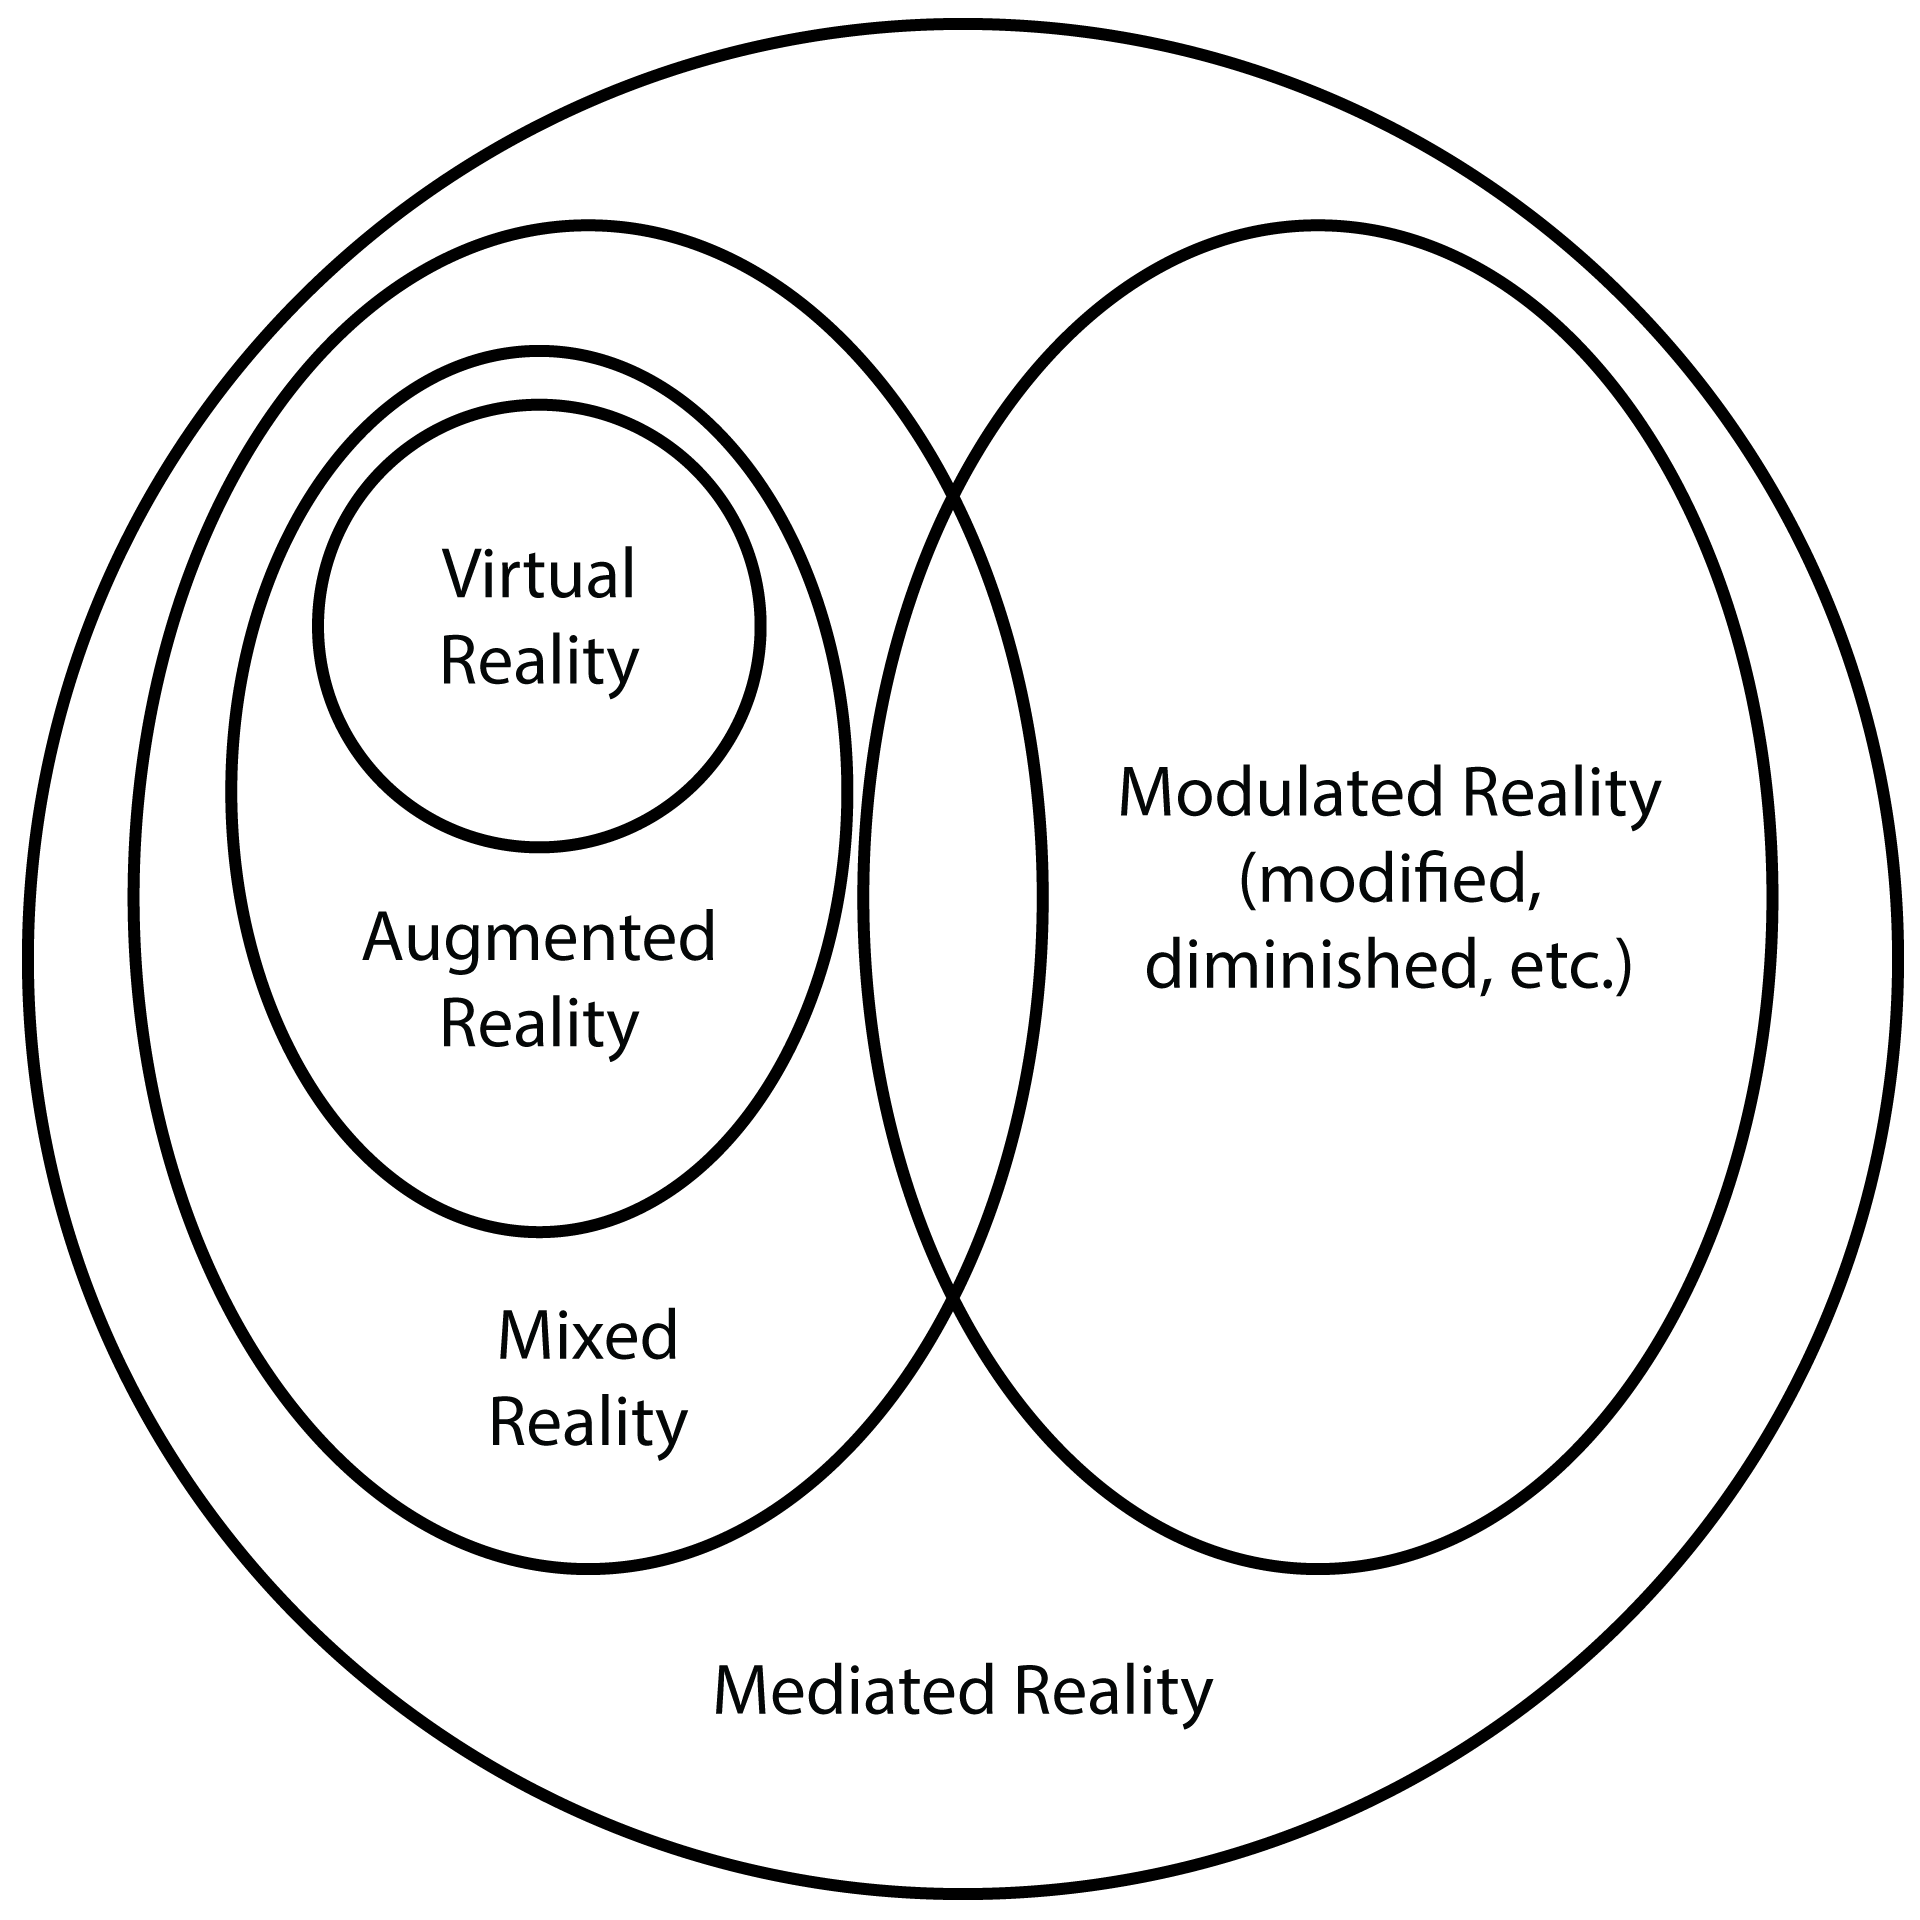
\includegraphics[width=0.95\linewidth]{Mann_venn_original.png}
  \caption{Original Mann venn diagram.}
  \label{Mann_venn_original.png}
\end{minipage}%
\begin{minipage}{.5\textwidth}
  \centering
  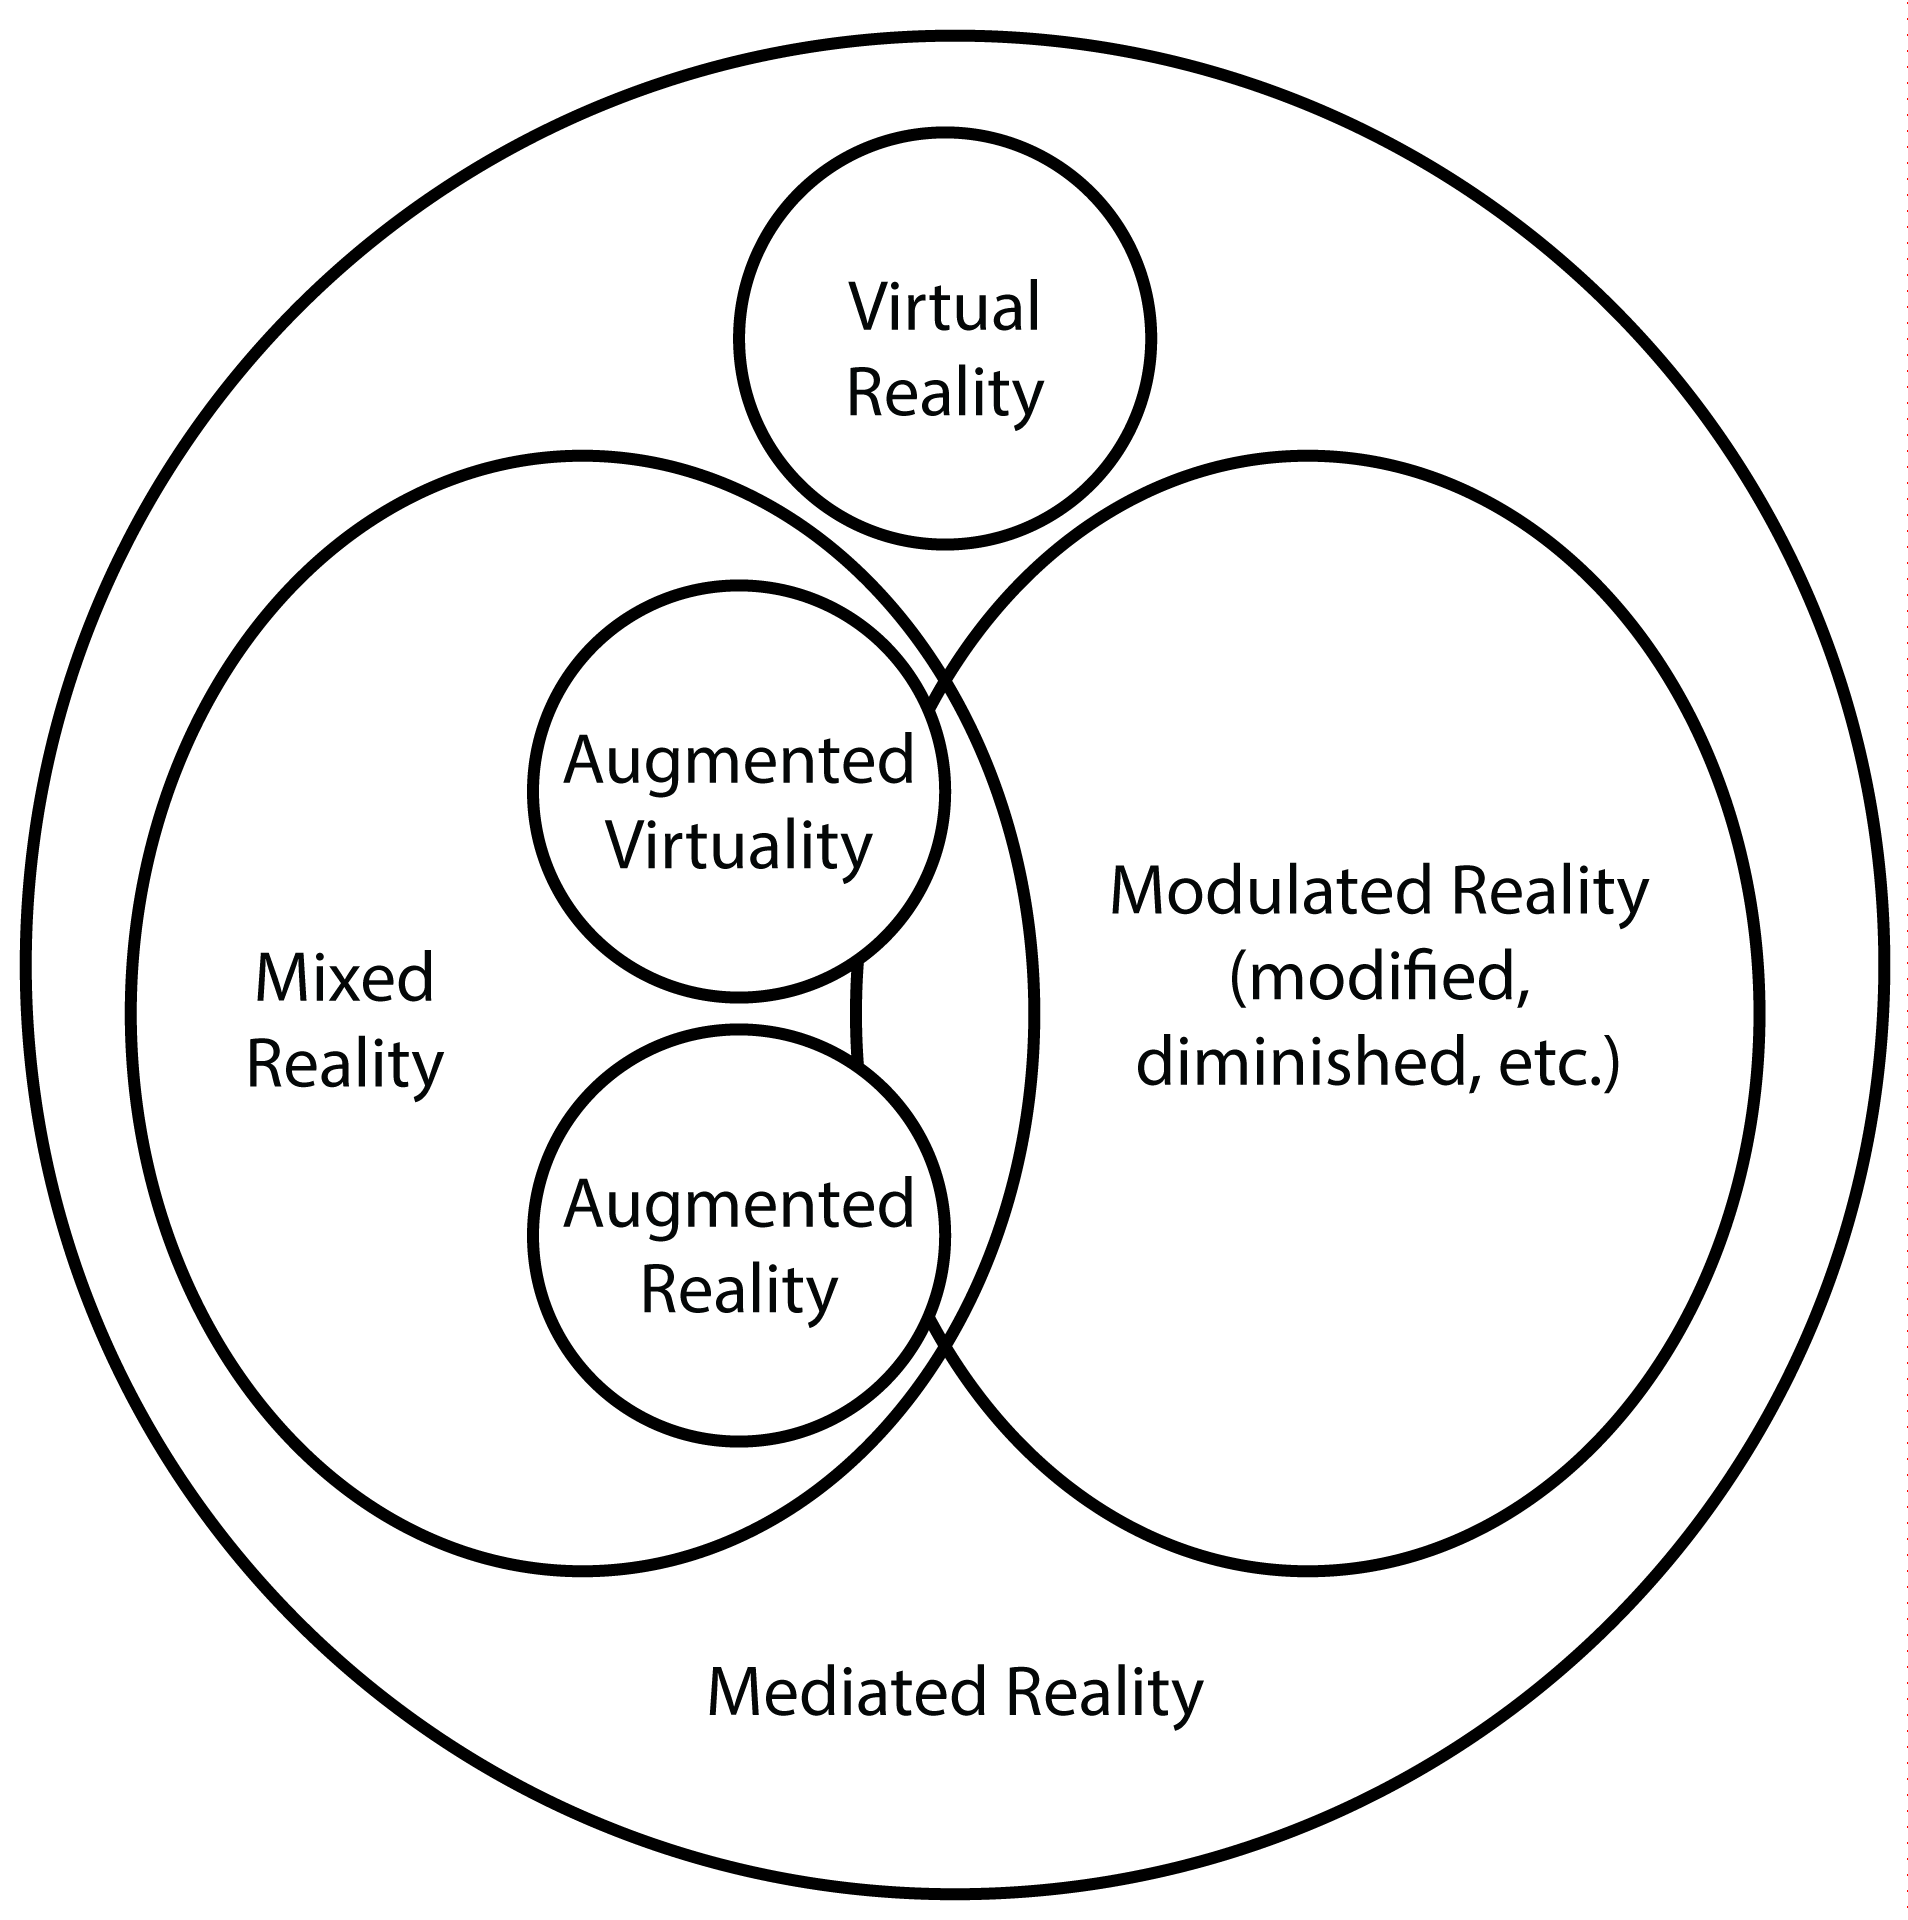
\includegraphics[width=0.95\linewidth]{Mann_venn_mod_1.png}
    \caption{Modified Mann venn diagram.}
    \label{Mann_venn_mod_1.png}
\end{minipage}
\end{figure}

Visualising the position of the `basic' classes of reality \& virtual reality using this same method requires more drastic alteration to the Venn diagram, but is diagnostic in further revealing the relationships between the terms introduced within Want's literature. The further modified Venn diagram (figure \ref{Mann_venn_mod_3.png}) shows;
\begin{itemize}
	\item mixed reality as the intersection of reality \& virtual reality;
	\item mediated reality can be comprised from purely real or purely virtual content;
	\item that all virtual reality is necessarily mediated;
	\item that modulated reality can comprise only mediated real, or both real \& virtual aspects in a mixed reality;
	\item that augmented reality \& augmented virtuality can feature in modulated reality systems.
\end{itemize}

\begin{figure}[h]
\centering
  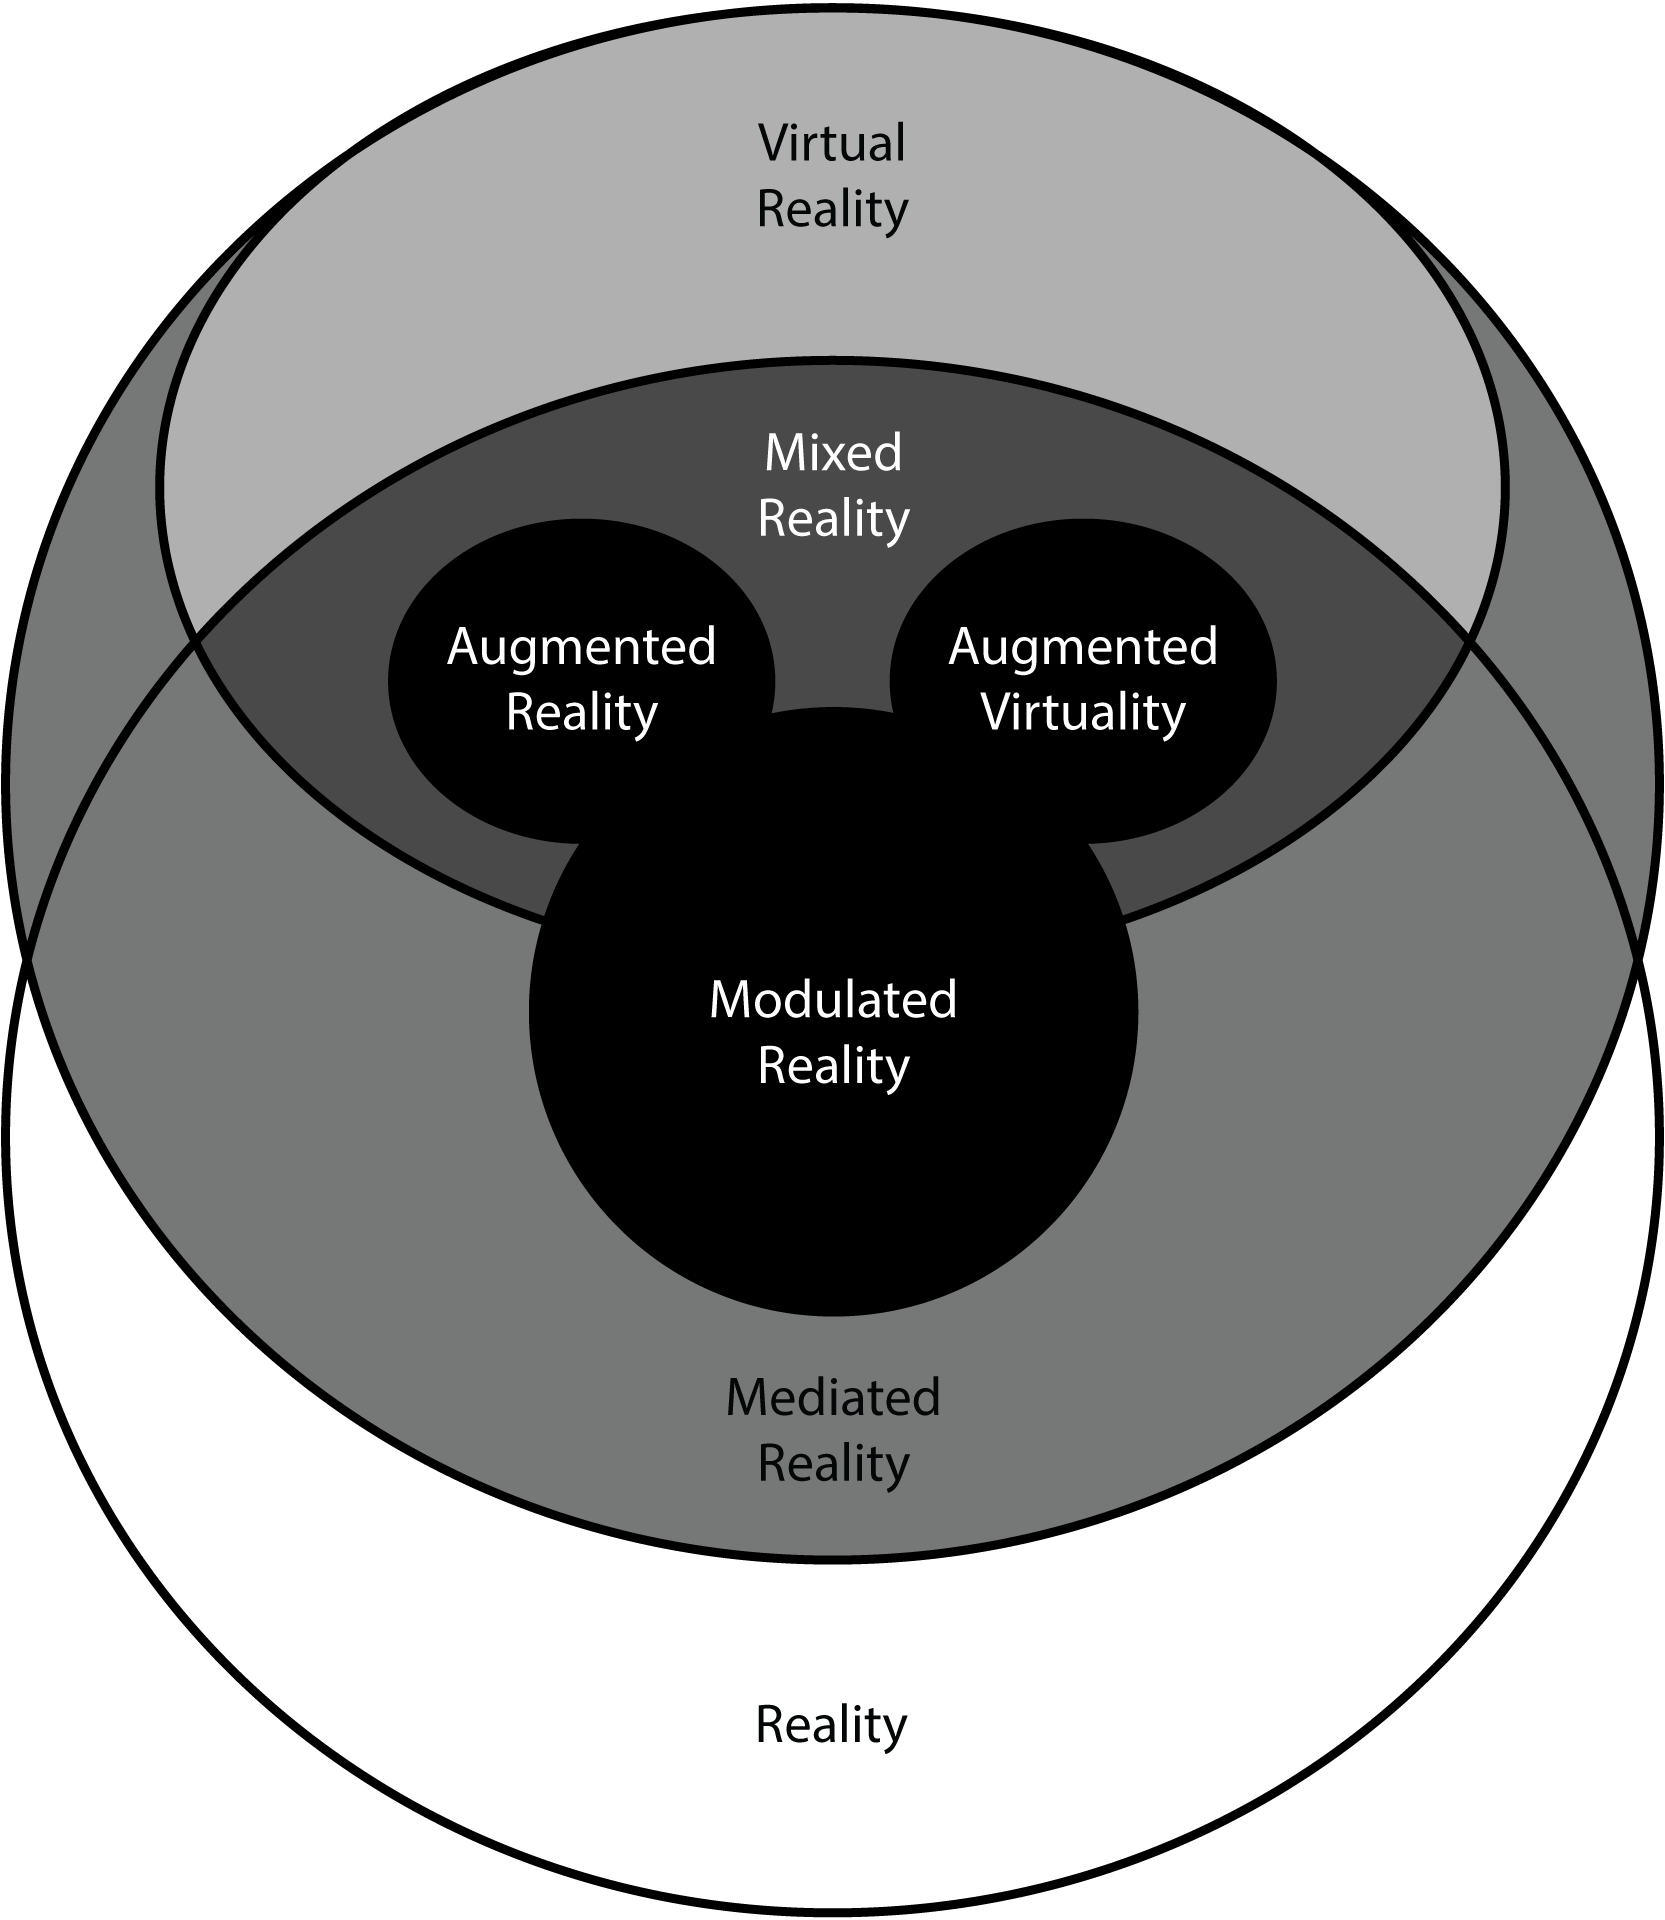
\includegraphics[width=0.5\linewidth]{Mann_venn_mod_3.png}
  \caption{Further modified Mann venn diagram.}
  \label{Mann_venn_mod_3.png}
\end{figure}

\textbf{Does this final Venn diagram not show that Modulated Reality can exist as Mixed Reality but which *isn't* either Augmented Reality or Augmented Virtuality though?}

\textbf{Also, what about a device that modulates a purely virtual view? Does that mean there should be an intersection between modulated reality \& virtual reality that *isn't* within the realm of mixed reality? Or does modulation of a wholly virtual environment not really count, as the content is by its very definition `modulated' by the fact it is not real?}

%=========================================================================================================
%=========================================================================================================

\section{Adopted Definitions of Alternate Realities}

Following are the definitions \& identifying/classifying criteria for the different categories of alternate realities identified thus far in this chapter.

%This review has discovered differing (and in some cases conflicting) definitions for the different categories of alternate realities and for the criteria for differentiating between them. What follows in this section represents the definitions and differentiating criteria that this review has adopted after concluding them the most widely accepted and well reasoned.

%=========================================================================================================

\begin{center}
\begin{longtable}{| l | p{12cm} |}

\hline	
	
%=========================================================================================================
		
\textbf{Reality} & An environment that is entirely unmodelled, with the viewport containing no virtual objects and with no computer-based quantitative information associated with any of the (necessarily real) objects. \\
		
\hline
		
%=========================================================================================================
		
\textbf{Virtual Reality} & The polar opposite of \textit{reality}, an environment that consists solely of virtual objects, with computer-based quantitative information associated with all of them and between all of them, creating a completely synthetic world entirely discrete and separate from the real world; a new world that exists solely within the data structures of a computer. \textbf{***cite Milgram and Want***}

While traditional definitions of \textit{virtual reality} require the environment to be completely immersive, such that when involved with the environment the user is completely unaware of the real environment that surrounds them (eg by using Head Mounted Displays \& body tracking techniques to remove logical anchors to the real world~\cite{Druck2006}) the criteria adopted herein are less drastic, classifying the virtual environments presented by video games viewed via 2D monitors as rudimentary implementations of virtual reality; they are completely modelled environments that exist entirely separate to the real world. \\
		
\hline
		
%=========================================================================================================

\textbf{Mixed Reality} & The broad range of environments that arise from the merging of real and virtual environments to some extent such that the result is neither entirely real nor entirely virtual, where real and virtual objects co-exist. Both \textit{augmented reality} and \textit{augmented virtuality} are included under the broader classification of \textit{mixed reality}. \\

\hline
		
%=========================================================================================================

\textbf{Augmented Reality} & A mixed reality environment comprising a real environment has had virtual objects added to or overlain upon it. A common approach for achieving this addition/overlay is superimposing virtual objects over a direct or indirect view of the real environment using Head Mounted Displays \&/or cameras~\cite{Krevelen2010}. \textbf{***better citation here pls, there was that big AR survey paper***} \\

	%A commercial example of \textit{augmented reality} is the Layar browser for mobile phones, which overlays various forms of data onto the view captured by a phone's camera after determining its location and orientation using GPS, accelerometer and magnetometer readings~\cite{eishita:layar}

%~\cite{Milgram1999}

\hline

%=========================================================================================================

\textbf{Augmented Virtuality} & A virtual environment upon which sampled real objects are overlain, perhaps through the use of cameras~\cite{caballero:behand}. \\

%A simple commercial example of augmented virtuality is the EyeToy accessory and associated software for Sony's Playstation 2 games console (and later the Playstation Eye for the Playstation 3), a digital camera that captures images of players and their surroundings and integrates them into the gaming experience presented on the screen.

\hline

%=========================================================================================================

\textbf{Mediated Reality} & \textit{``A general framework for artificial modification of human perception by way of devices for augmenting, deliberately diminishing, and more generally, for otherwise altering sensory input''}~\cite{Mann2002a}. Encompasses all of mixed reality \& modulated reality. \\

\hline

%=========================================================================================================

\textbf{Modulated Reality} & Platforms that aim to modify the user's view, by multiplicative, diminishing, rotational, etc. techniques, where the user's view can be wholly real, or a mix of real \& virtual content. \\

%=========================================================================================================

\textbf{HyperReality} &  \\

%=========================================================================================================

\hline

\end{longtable}
\end{center}

%=========================================================================================================
%=========================================================================================================


``HyperReality (HR) is a hypothetical communications infrastructure made possible by information technology. It allows the commingling of physical reality with virtual reality and human intelligence with artificial intelligence.''

``HyperReality (HR) is a technological capability, like nanotechnology, human cloning and artificial intelligence. Like them, it does not as yet exist in the sense of being clearly demonstrable and publicly available. Like them, it is maturing in laboratories where the question `if?' has been replaced by `when?' And like them, the implications of its appearance as a basic infrastructure technology are profound and merit careful consideration.''

``The concept of HyperReality (HR), like the concepts of nanotechnology, cloning and artificial intelligence, is in principle very simple. It is nothing more than the technological capability to intermix virtual reality (VR) with physical reality (PR) and artificial intelligence (AI) with human intelligence (HI) in a way that appears seamless and allows interaction.''

``The project that led to the concept of HR began with the idea of teleconferencing in virtual reality.

ATR (Advanced Telecommunications Research) in Kansai Science City

``HyperReality is a technological capability that makes possible the seamless integration of physical reality and virtual reality, human intelligence and artificial intelligence.''

Must be seamless, without a `bezel' (HyperReality p142)

``HR makes ir possible for the physically real inhabitants of one place to purposively coact with the inhabitants of remote locations as welll as with computer-generated imaginary or artificial life forms in a HyperWorld.

Distributed Virtual Reality - simply shared VR that is accessible by multiple simultaneous users via telecommunications infrastructure (HyperReality p13)

HR is a single mixed reality environment (HyperReality p26)

``It seeks to make virtual reality something that is experienced as part of physical reality, so that virtual and real phenomena appear to interact with each other: HR is VR \textit{as well as, not instead of,} PR.'' (HyperReality p31, emphasis original)

HyperReality is a technological metaconcept (HyperReality p41)

HyperReality is a technology that enables hyperreality (the postmodern term) (HyperReality p41)

``HyperReality means a reality in which there is the extra dimension of virtual reality within normal physical reality'' (HyperReality p42)

``The implication of HR is that, wherever you are, you could be somewhere else.'' (HyperReality p149) - not sure I agree with this as definition of HR though, as HR is about VR *as well as* rather than instead of PR - my mobile parallel reality is more like VR instead of PR, but with the ability of rapidly temporal change in which is being observed.




From Simulacra and Simulation (Jean Baudrillard), Hyperreality is essentially an inability of consciousness to distinguish reality from a simulation of reality. Hyperreality is seen as a condition in which what is real and what is fiction are seamlessly blended together so that there is no clear distinction between where one ends and the other begins. It allows the commingling of physical reality with virtual reality (VR) and human intelligence with artificial intelligence (AI).




\section{Cross Reality}

Cross reality is the ubiquitous mixed reality situation that arises from the fusion of real-world sensor/actuator infrastructure with virtual environments, such that augmented reality and augmented virtuality manifest simultaneously and facilitate synchronous multi-directional exchange of media and control information between real and virtual environments. Sensors collect and tunnel dense real-world data into virtual environments where they are interpreted and displayed to dispersed users, whilst interaction of virtual participants simultaneously incarnates into the real world through a plenitude of diverse displays and actuators~\cite{Paradiso2009}.

The principle features that distinguish cross reality from the other alternate realities covered by this chapter are;
\begin{enumerate}
	\item a shift from single- to bi-directional information flow between real and virtual environments~\cite{kim:practical}
	\item that both environments are complete unto themselves (but are enriched by their ability to mutually reflect, influence and merge into one another).~\cite{lifton:merging}
\end{enumerate}

\textit{This thesis presents systems that focus on the second aspect above \& extends it by permitting both environments to be experienced at any time \& position.}

%=========================================================================================================

\subsection{The History of Cross Reality}

Cross reality was realised \& developed as a research area by the Responsive Environments Group at MIT's Media Lab, centred around the research of Joshua Lifton~\cite{Lifton2007a} in combining the Plug sensor/actuator platform~\cite{Lifton2007b} with a Second Life hosted virtual model of the physical Lab in the `Shadow Lab' project. These projects furthered initial work by the IBM Virtual Universe Community~\cite{Hughes2006, Hughes2006a,Hughes2006b}, whose progress toward a cross reality platform was confirmed via personal correspondence;

\begin{quote}
\textit{``The control mechanisms worked two ways generally. There was a physical lab that had devices that were controlled by a pub/sub mechanism based on the light weight protocol MQTT. Those devices subscribed to various messages. So initially web pages controlled them \ldots\ Equally the objects generated messages when they were physically switched on and off. As SL had an RPC interface it was possible \ldots\ to subscribe to the same messages and send requests into SL to change states of object \ldots\ So there were lights, blinds, proximity detectors and even the tilt sensors on the laptops that were instrumented with these messages.''}
\end{quote}

\begin{figure}[h]
\centering
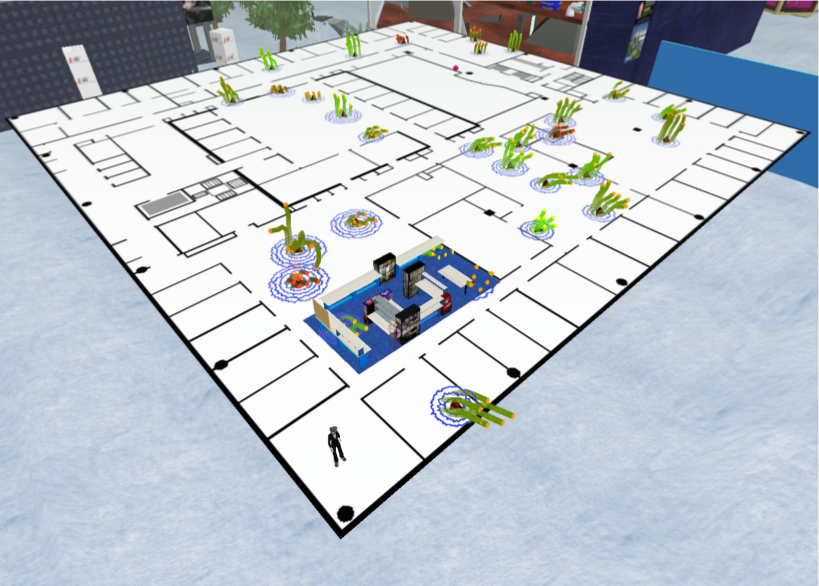
\includegraphics[width=\textwidth]{lifton_shadow_lab.png}
\caption{Side view of the Shadow Lab platform, showing a reconstruction of part of the Media Lab, virtual `data ponds' where Plug sensor/actuator devices were place \& a human-sized avatar.}
\label{lifton_shadow_lab.png}
\end{figure}

The Shadow Lab did not allow for tandem visual engagement with both constituent environments of the cross reality platform.

The Ubiquitous Sensor Portal project that followed the Dual Reality Lab partially addressed this, by situating 45 I/O rich `portals', shown in figure \ref{ubiquitous_sensor_portal.jpg}, throughout the Media Lab, each with a corresponding extension in Second Life. However in stark contrast to the Dual Reality Lab, the virtual portals were not situated in a simulation of the real Media Lab in situations corresponding to their physical location, but instead used a more abstract virtual representation with a geometric layout; this design, shown in figure \ref{ubiquitous_sensor_portal_virtual.png}, reflected intellectual affiliation as opposed to real-world locationHowever in stark contrast to the Dual Reality Lab, the virtual portals were not situated in a simulation of the real Media Lab in situations corresponding to their physical location, but instead used a more abstract virtual representation with a geometric layout; this design, shown in figure \ref{ubiquitous_sensor_portal_virtual.png}, reflected intellectual affiliation as opposed to real-world location

\begin{figure}[h]
\centering
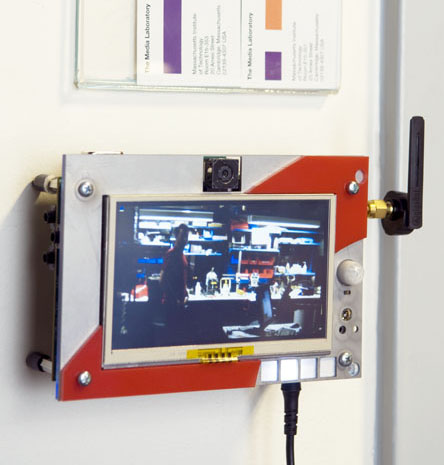
\includegraphics[width=0.6\textwidth]{ubiquitous_sensor_portal.jpg}
\caption{A Ubiquitous Sensor Portal.}
\label{ubiquitous_sensor_portal.jpg}
\end{figure}

%=========================================================================================================

\subsection{The Vacancy Problem}

Lifton identifies the `vacancy problem';
\begin{quote}
\textit{``the noticeable and profound absence of a person from one world, either real or virtual, while they are participating in the other. Simply put, the vacancy problem arises because people do not currently have the means to be in more than one place (reality) at a time.''}
\end{quote}
as a fundamental characteristic of the current generation of virtual worlds and proposes dual reality, more closely linking the real world with the virtual world, as an approach to mitigate the problem.

\textbf{See HyperReality p35}

%=========================================================================================================

\subsection{Lifton's Virtual Worlds Taxonomy}

As the prominent figure in the development of the cross reality paradigm it is worth comparing Joshua Lifton's definitions for different categories of alternate realities and the relationships between them~\cite{Lifton2007a} in the current context.

Lifton's definitions, or more accurately his relationships between, the terms \textit{reality}, \textit{augmented reality}, \textit{mixed reality} and \textit{virtual reality} do not perfectly match the consensus that this review has observed. Lifton defines the terms individually in agreement with the consensus, however doesn't proffer the conclusion that mixed reality is a broad term that includes augmented reality. He also doesn't mention augmented virtuality, even though his cross reality projects could be construed as implementing it. Finally his diagram that alludes to Milgram's continua and is included as figure \ref{original_lifton_axis.png}, situates mixed reality at an incorrect position, implying that Lifton's definition of mixed reality is of a discrete state to that of augmented reality, even though his textual definition of mixed reality hints that it logically encompasses augmented reality. This review presents a modified version of Lifton's diagram to illustrate these differences as figure \ref{modified_lifton_axis.png}.

Lifton does however explain that while such a taxonomy can be successfully applied to most alternate reality efforts, it does not well address the concept of cross reality where there are two complete realities, one real and one virtual. \textbf{***is there a direct citation for this?***}

\begin{figure}[h]
	\centering
	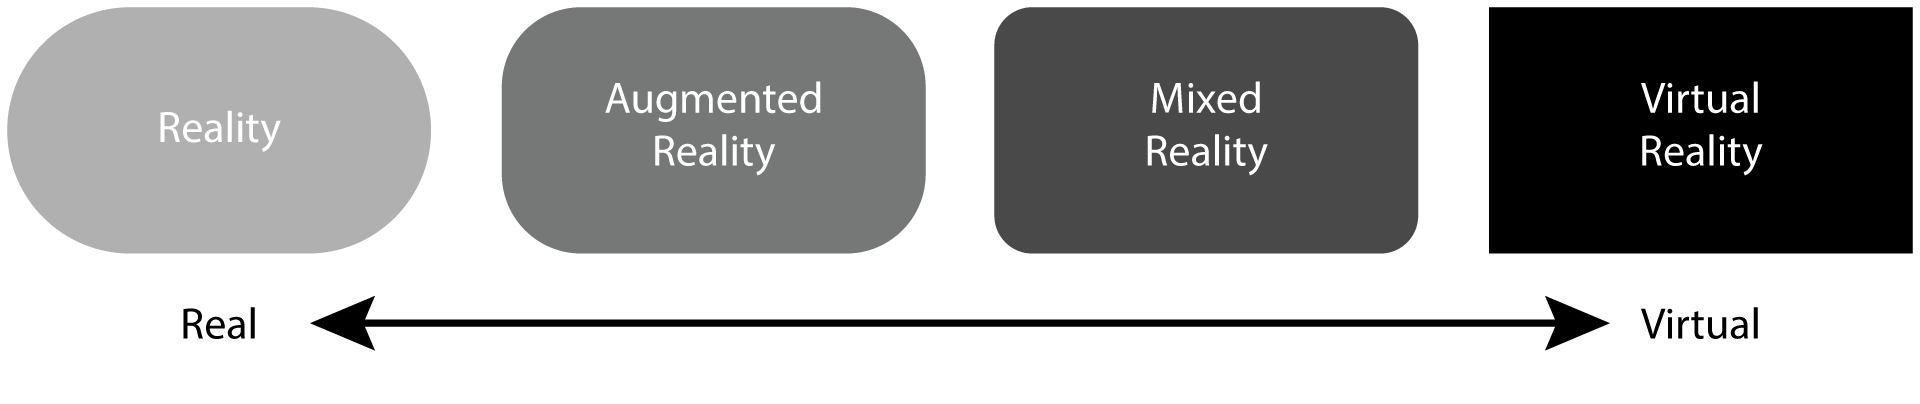
\includegraphics[width=.8\textwidth]{Lifton_continuum_original.png}
	\caption{The \textit{``virtual worlds taxonomy as viewed on the real-virtual axis''} presented by Lifton.}
	\label{original_lifton_axis.png}
\end{figure}

\begin{figure}[h]
	\centering
	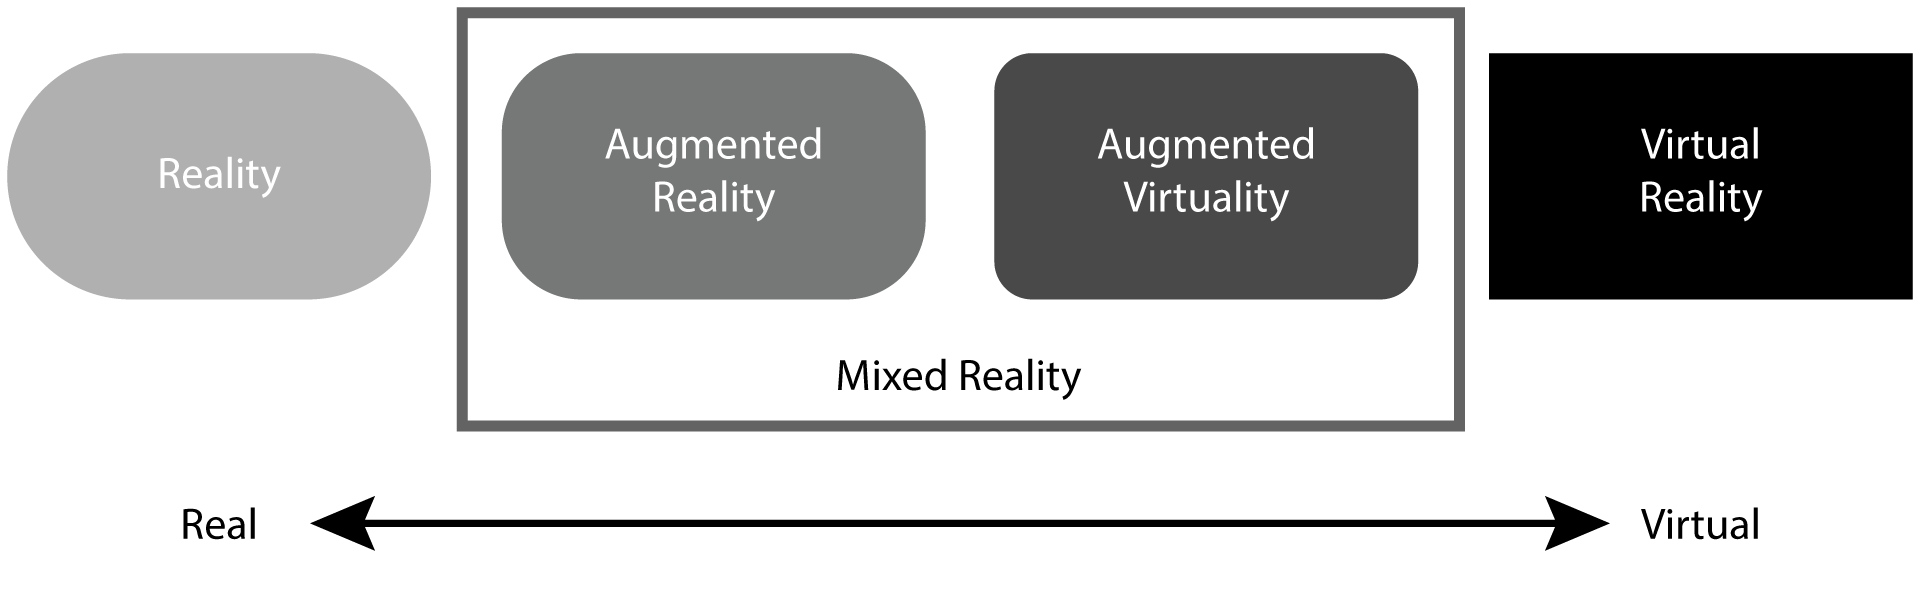
\includegraphics[width=.8\textwidth]{Lifton_continuum_modified.png}
	\caption{Lifton's taxonomy as modified by this review.}
	\label{modified_lifton_axis.png}
\end{figure}

%=========================================================================================================

\clearpage

\subsection{Cross Reality \& Milgram \& Kishino's Reality-Virtuality Continuum}

The position of XR in relation to other alternate realities studied by Computer Science can be visualised using Milgram \& Kishino's \textit{virtuality continuum} that stretches from an entirely real environment at one extreme to an ontologically parallel but entirely virtual environment~\cite{Qvortrup2002} at the other. The explanation herein distinguishes between environments themselves (depicted in figures \ref{virtuality-continuum-augmented-reality} to \ref{virtuality-continuum-cross-reality-3} by solid ellipses) \& where the stimuli that the user is perceiving originate from (depicted by dashed ellipses).

%Ontology - The core meaning within computer science is a model for describing the world that consists of a set of types, properties, and relationship types. There is also generally an expectation that the features of the model in an ontology should closely resemble the real world (related to the object).

Of particular importance is to appreciate the distinction between a XR system \& an \textit{augmented reality} (AR) system, as both concepts involve user engagement with both real \& virtual content. Whilst an AR system features a single environment, comprised of the user's RW overlain by some virtual content, with the user perceiving stimuli from this single augmented environment (figure \ref{virtuality-continuum-augmented-reality}), a XR system instead features two discrete environments, one real \& the other virtual, each complete unto itself (figure \ref{virtuality-continuum-cross-reality-1}).

Whilst AR falls within the realms of Mixed Reality (MR), a XR system can be considered as occupying the two extremes of the continuum outwith the MR region. However, XR systems that allow simultaneous interaction with both of their constituent environments blur this definition; using a XR platform such as that discussed in this document, a user can transition between perceiving stimuli from each of these environments (figures \ref{virtuality-continuum-cross-reality-2} \& \ref{virtuality-continuum-cross-reality-3}) in a manner that allows them to engage with each environment without becoming wholly vacant from the other.

\begin{figure}[h]
	\begin{center}
		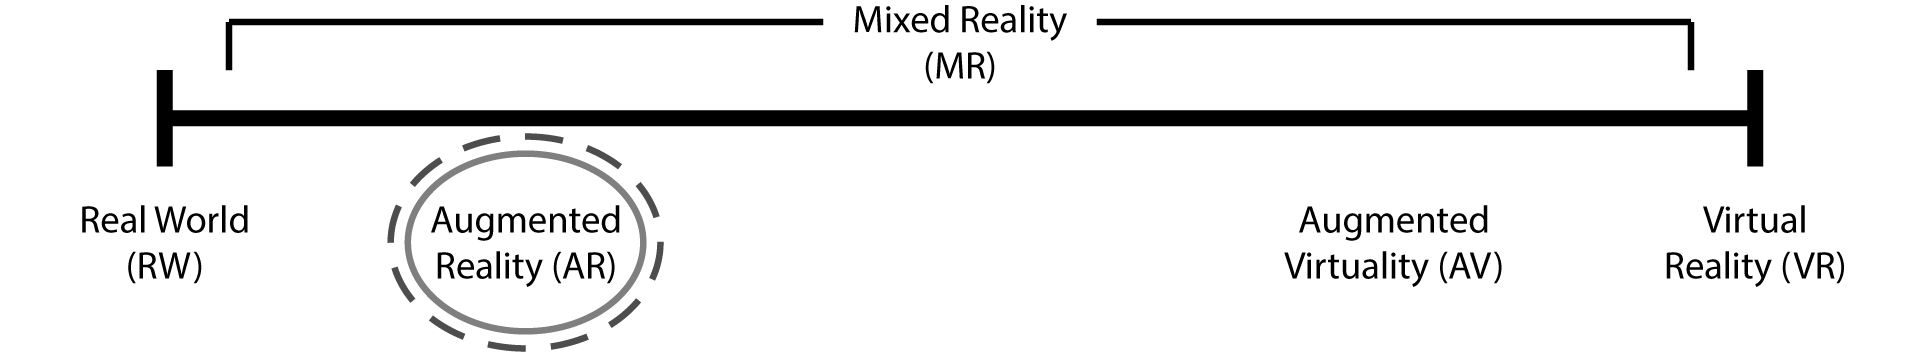
\includegraphics[width=\textwidth]{virtuality-continuum-augmented-reality.png}
		\caption{AR visualised using the virtuality continuum.}
		\label{virtuality-continuum-augmented-reality}
	\end{center}
\end{figure}

\begin{figure}[h]
	\begin{center}
		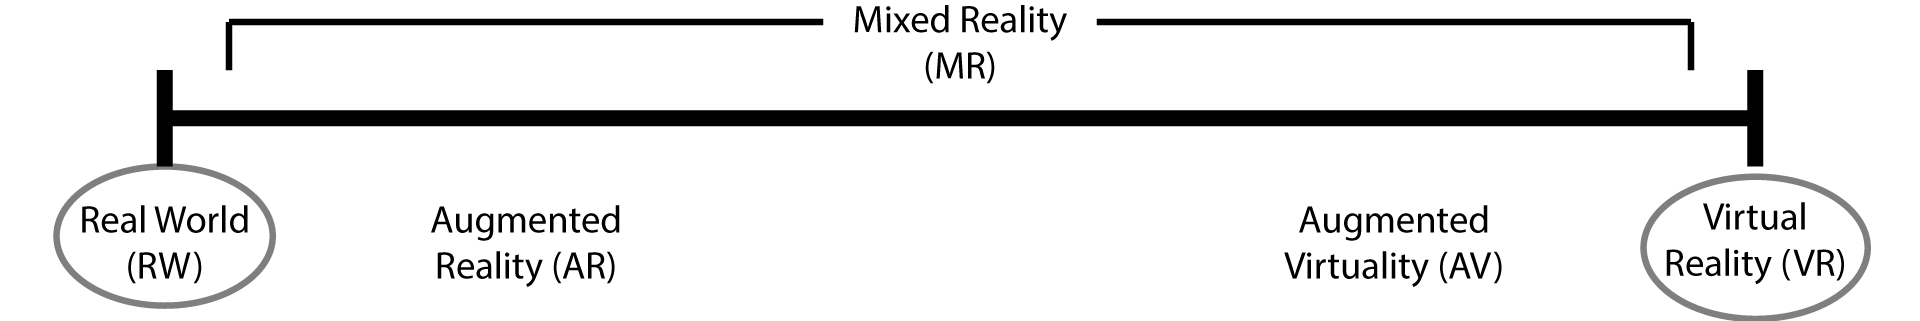
\includegraphics[width=\textwidth]{virtuality-continuum-cross-reality-1.png}
		\caption{The two environments that comprise a XR system.}
		\label{virtuality-continuum-cross-reality-1}
	\end{center}
\end{figure}

\textbf{Is it worth pointing out on the diagram that a true XR system would have a constant bi-directional stream of data between the two environments? And that without this, we have something like parallel reality?}

\begin{figure}[h]
	\begin{center}
		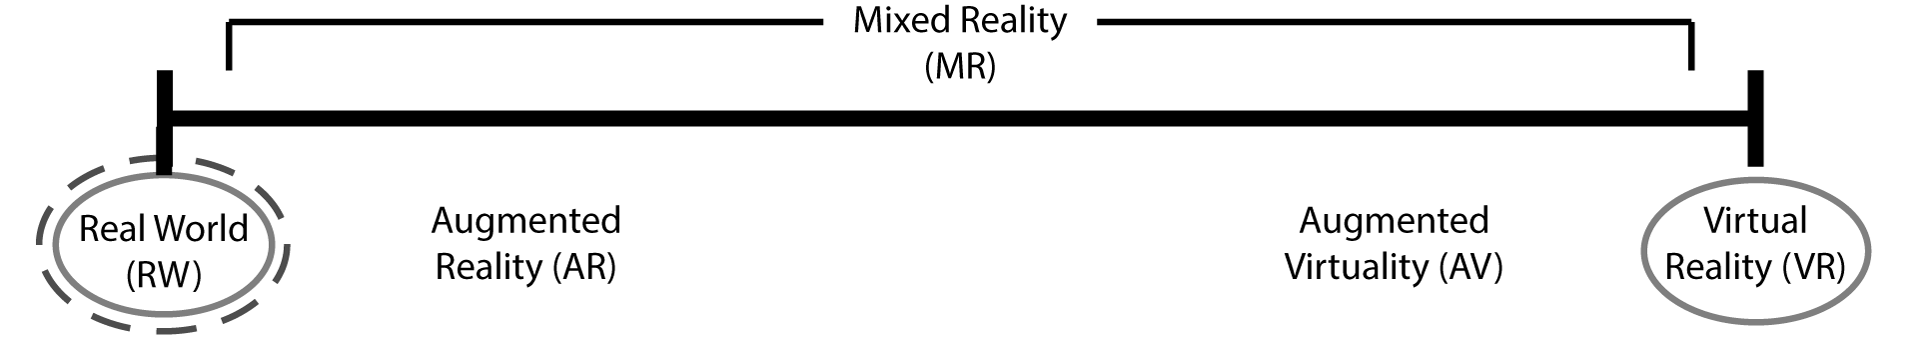
\includegraphics[width=\textwidth]{virtuality-continuum-cross-reality-2.png}
		\caption{A XR system with the user attending to RW stimuli.}
		\label{virtuality-continuum-cross-reality-2}
	\end{center}
\end{figure}

\begin{figure}[h]
	\begin{center}
		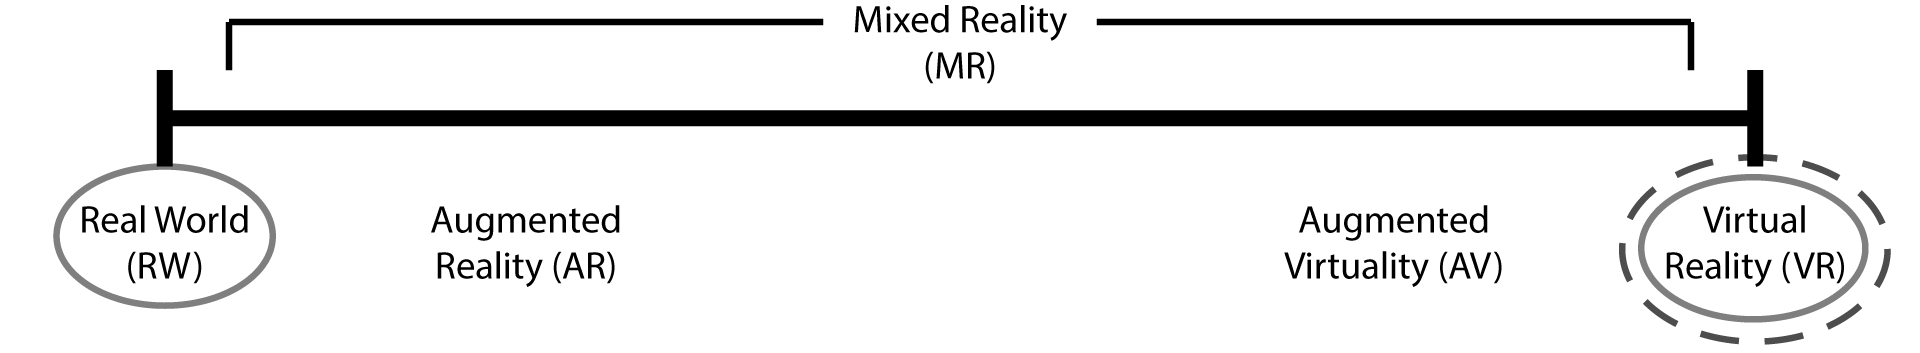
\includegraphics[width=\textwidth]{virtuality-continuum-cross-reality-3.png}
		\caption{A XR system with the user attending to VR stimuli.}
		\label{virtuality-continuum-cross-reality-3}
	\end{center}
\end{figure}

\begin{figure}[h]
	\begin{center}
		
\includegraphics[width=\textwidth]{virtuality-continuum-cross-reality-information-flows-dashed.png}
		\caption{The two environments that comprise a XR system, plus the bidirectional information flow between them.}
	\end{center}
\end{figure}

%=========================================================================================================

\subsection{PolySocial Reality in Cross Reality Systems}

\textbf{Some references from HyperReality}

%=========================================================================================================
%=========================================================================================================

\section{On Presence}

\subsection{Combined Milgram \& Kishino continuum/Waterworth \& Waterworth three dimensions of virtual experience model}

\newcommand{\presencefootnote}{\footnote{\textbf{Presence} in this context is defined as a state of heightened perceptual processing of environmental stimuli (\textit{``a psychological focus on direct perceptual processing''}~\cite{Waterworth2001}) accompanied by lessened conceptual reasoning, whether these environmental stimuli originate from a real environment, a virtual environment, a mixed reality environment, or even from multiple discrete environments.}}

\newcommand{\absencefootnote}{\footnote{\textbf{Absence} is defined as \textit{``a psychological focus on \ldots conceptual processing''}~\cite{Waterworth2001}.}}

The virtuality continuum is here considered to be analogous to the \textit{locus of attention} axis of Waterworth \& Waterworth's \textit{three dimensions of virtual experience} model~\cite{Waterworth2001}; the combination of these models is shown by figure \ref{focus-locus-sensus-with-virtuality-continuum}. In this model, locus of attention represents the environment where the stimuli that the user is perceiving originate from; focus of attention represents the balance between conceptual/abstract reasoning \& perceptual/concrete processing, where complex conceptual reasoning results in little attention being paid to processing environmental percepts (whether originating from real or virtual stimuli) thus reducing presence\presencefootnote{} in that environment toward its antithesis $-$ absence\absencefootnote{}; and sensus of attention represents the level of conscious arousal (or `wakefulness'~\cite{Laureys2009}) of the user, whether directed toward percepts originating from real stimuli, virtual stimuli, a mix, or not directed toward any percepts in the case of completely `absent' conceptual reasoning.

\begin{figure}[h]
	\begin{center}
		
\includegraphics[width=0.7\textwidth]{focus-locus-sensus-with-virtuality-continuum.png}
		\caption{The combined virtuality continuum/three dimensions of virtual experience model.}
		\label{focus-locus-sensus-with-virtuality-continuum}
	\end{center}	
\end{figure}

%The Sensus Dimension - the importance of being awake in class
%"Even as we sleep dreamlessly..." (example of being 'unconscious' in this regard)

%fourth axis is alterity, between hermeneutics \& embodiment

%=========================================================================================================
%=========================================================================================================

\section{Parallel Reality visualised using the combined model}

\newcommand{\breakinpresencefootnote}{\footnote{The definition of \textbf{break in presence} adopted herein is the second from Waterworth \& Waterworth~\cite{Waterworth2001} (p205): a movement along the focus axis away from presence in the real or a virtual environment \& toward absence. This differs to Slater \& Steed's original definition in~\cite{Slater2000} as they considered presence only in terms of attending to stimuli from a virtual environment, with a break in presence as a Gestalt switch to instead attending to stimuli from the real environment. Waterworth \& Waterworth's model considers presence in terms of attending to stimuli from either the real \textit{or a virtual} environment, with a break in presence representing absence in the sense of heightened conceptual load \& the resultant reduced perceptual processing of environmental stimuli originating from \textit{either} the real or a virtual environment. This definition better fits the situation invoked by the Mirrorshades platform, which is concerned with intentionally \& willingly switching engagement between stimuli from both real \& virtual environments, rather than engaging with stimuli from only a virtual environment in a scenario where stimuli from the real environment are considered a `distraction'.}}

The novel aspect of the Mirrorshades platform is the ability it imparts upon its user to switch their locus of attention between equivalent vantage points in RW \& VR environments whilst walking around. This is achieved by the user performing transitions between RW visual stimuli \& VR visual stimuli, both presented via their HMD. This extends existing XR research by allowing the user to engage with the visual stimuli of the VR component of a XR system from any position \& at any time.

In order to achieve the highest quality of experience with this style of interaction with XR systems, it is vital to determine how best to implement these transitions; that is, to mitigate the increased cognitive load (manifesting as increased conceptual reasoning \& reduced perceptual processing, see section \ref{waterworth}) required to comprehend these transitions, as this increased cognitive load will detract from engagement with the environments \& reduce the user's willingness to perform these transitions.

Whilst some researchers support the notion that in systems where more than one environment competes for the user's locus of attention there is an `all or nothing' Gestalt switch between awareness of one environment \& the other~\cite{Slater2002}, which would result in a substantial increase in cognitive load upon each transition, Mirrorshades has been developed in support of the contrary opinion; that switching locus of attention from the stimuli of one environment to those of another does not completely overrule the user's awareness of the former, that both environments can be perceived at the same time (albeit one to a lesser extent)~\cite{Ijsselsteijn2001} \& that when engaging with VR content a user's focus can even be said to typically be \textit{shared} between VR \& RW~\cite{Waterworth2001}.

This latter position is particularly apt for situations wherein the RW \& VR environments share the same fundamental layout \& dimensions, as those in a XR system often do, as the inherent familiarity between the two environments reduces the cognitive load associated with transitioning between them. Furthermore, the notion of experience of presence as changing continually from moment-to-moment~\cite{Heeter2003, Ijsselsteijn1998} lends confidence to the successful mitigation of the cognitive load associated with these transitions to manageable levels. One might even liken this `switching' between RW \& VR to the `cycling through' behaviour observed in users of virtual communities, which stemmed from the `window' concept of modern computer operating systems~\cite{Turkle2004}.

However, no matter how smooth the transition the process is expected to always result in some heightened cognitive load, a temporary \textit{break in presence}\breakinpresencefootnote{} (BIP), as the user comes to terms with the new environment presented to them \& comprehends its relation to the other environment that they were just perceiving.

%\section{Transitions}
Transitions can be performed in multiple different manners \& it is hypothesized that users will prefer different styles of transition in different situations, surroundings \& scenarios (where `preference' toward a particular style of transition is expected to correlate strongly with a less severe BIP being experienced upon its execution).

To this end, several different transition methods have been developed \& this investigation will endeavour to identify \& quantify preferences toward them, to infer which approaches to transitioning between RW \& VR visual stimuli are more or less appropriate for the different situations that arise where a platform like Mirrorshades may be deployed. In particular, it is hypothesized that there will be a strong correlation between participant movement (or lack thereof) \& choice of particular transition style.

\subsection{Transitions using the Combined Model}
Visualised using the combined model (see section \ref{waterworth}) as figure \ref{focus-locus-sensus-with-virtuality-continuum-with-transition}, these transitions are an oscillation along the locus axis, between a RW environment at one position \& a VR environment at the other.

Heightened cognitive load required to comprehend a transition is a temporary movement upon the focus axis from presence toward absence (a BIP). With the ability of a wide FOV, stereoscopic 3D, head-tracked HMD to produce immersive VR visual stimuli that require fairly limited cognitive processing \& our inherent ability to engage with our RW surroundings without significant cognitive load, focus is expected to be high (toward the presence extremum) when attending to stimuli from either RW or VR.

Sensus is expected to be largely task dependent, however when performing a task that involves actively engaging with the visual stimuli from either/both of RW or VR it is expected to be high (toward the conscious extremum). Upon triggering a transition, sensus is expected to increase, as the user centres their attention upon relating the visual stimuli from the new environment to those they were just perceiving from the other environment

%Whilst continued exposure to the platform is expected to reduce the severity of the BIPs, mitigating their severity from the outset (reducing the displacement from the presence extremum downwards toward absence) through informed execution of the transitions between RW \& VR is believed to be important to the overall quality of experience that users receive.

%absent-mindedness - caused by increased attention toward a single object of focus (hyperfocus, eg the object of focus is the switch)
% or caused by distraction (again, the switch)

\begin{figure}[h]
	\begin{center}
		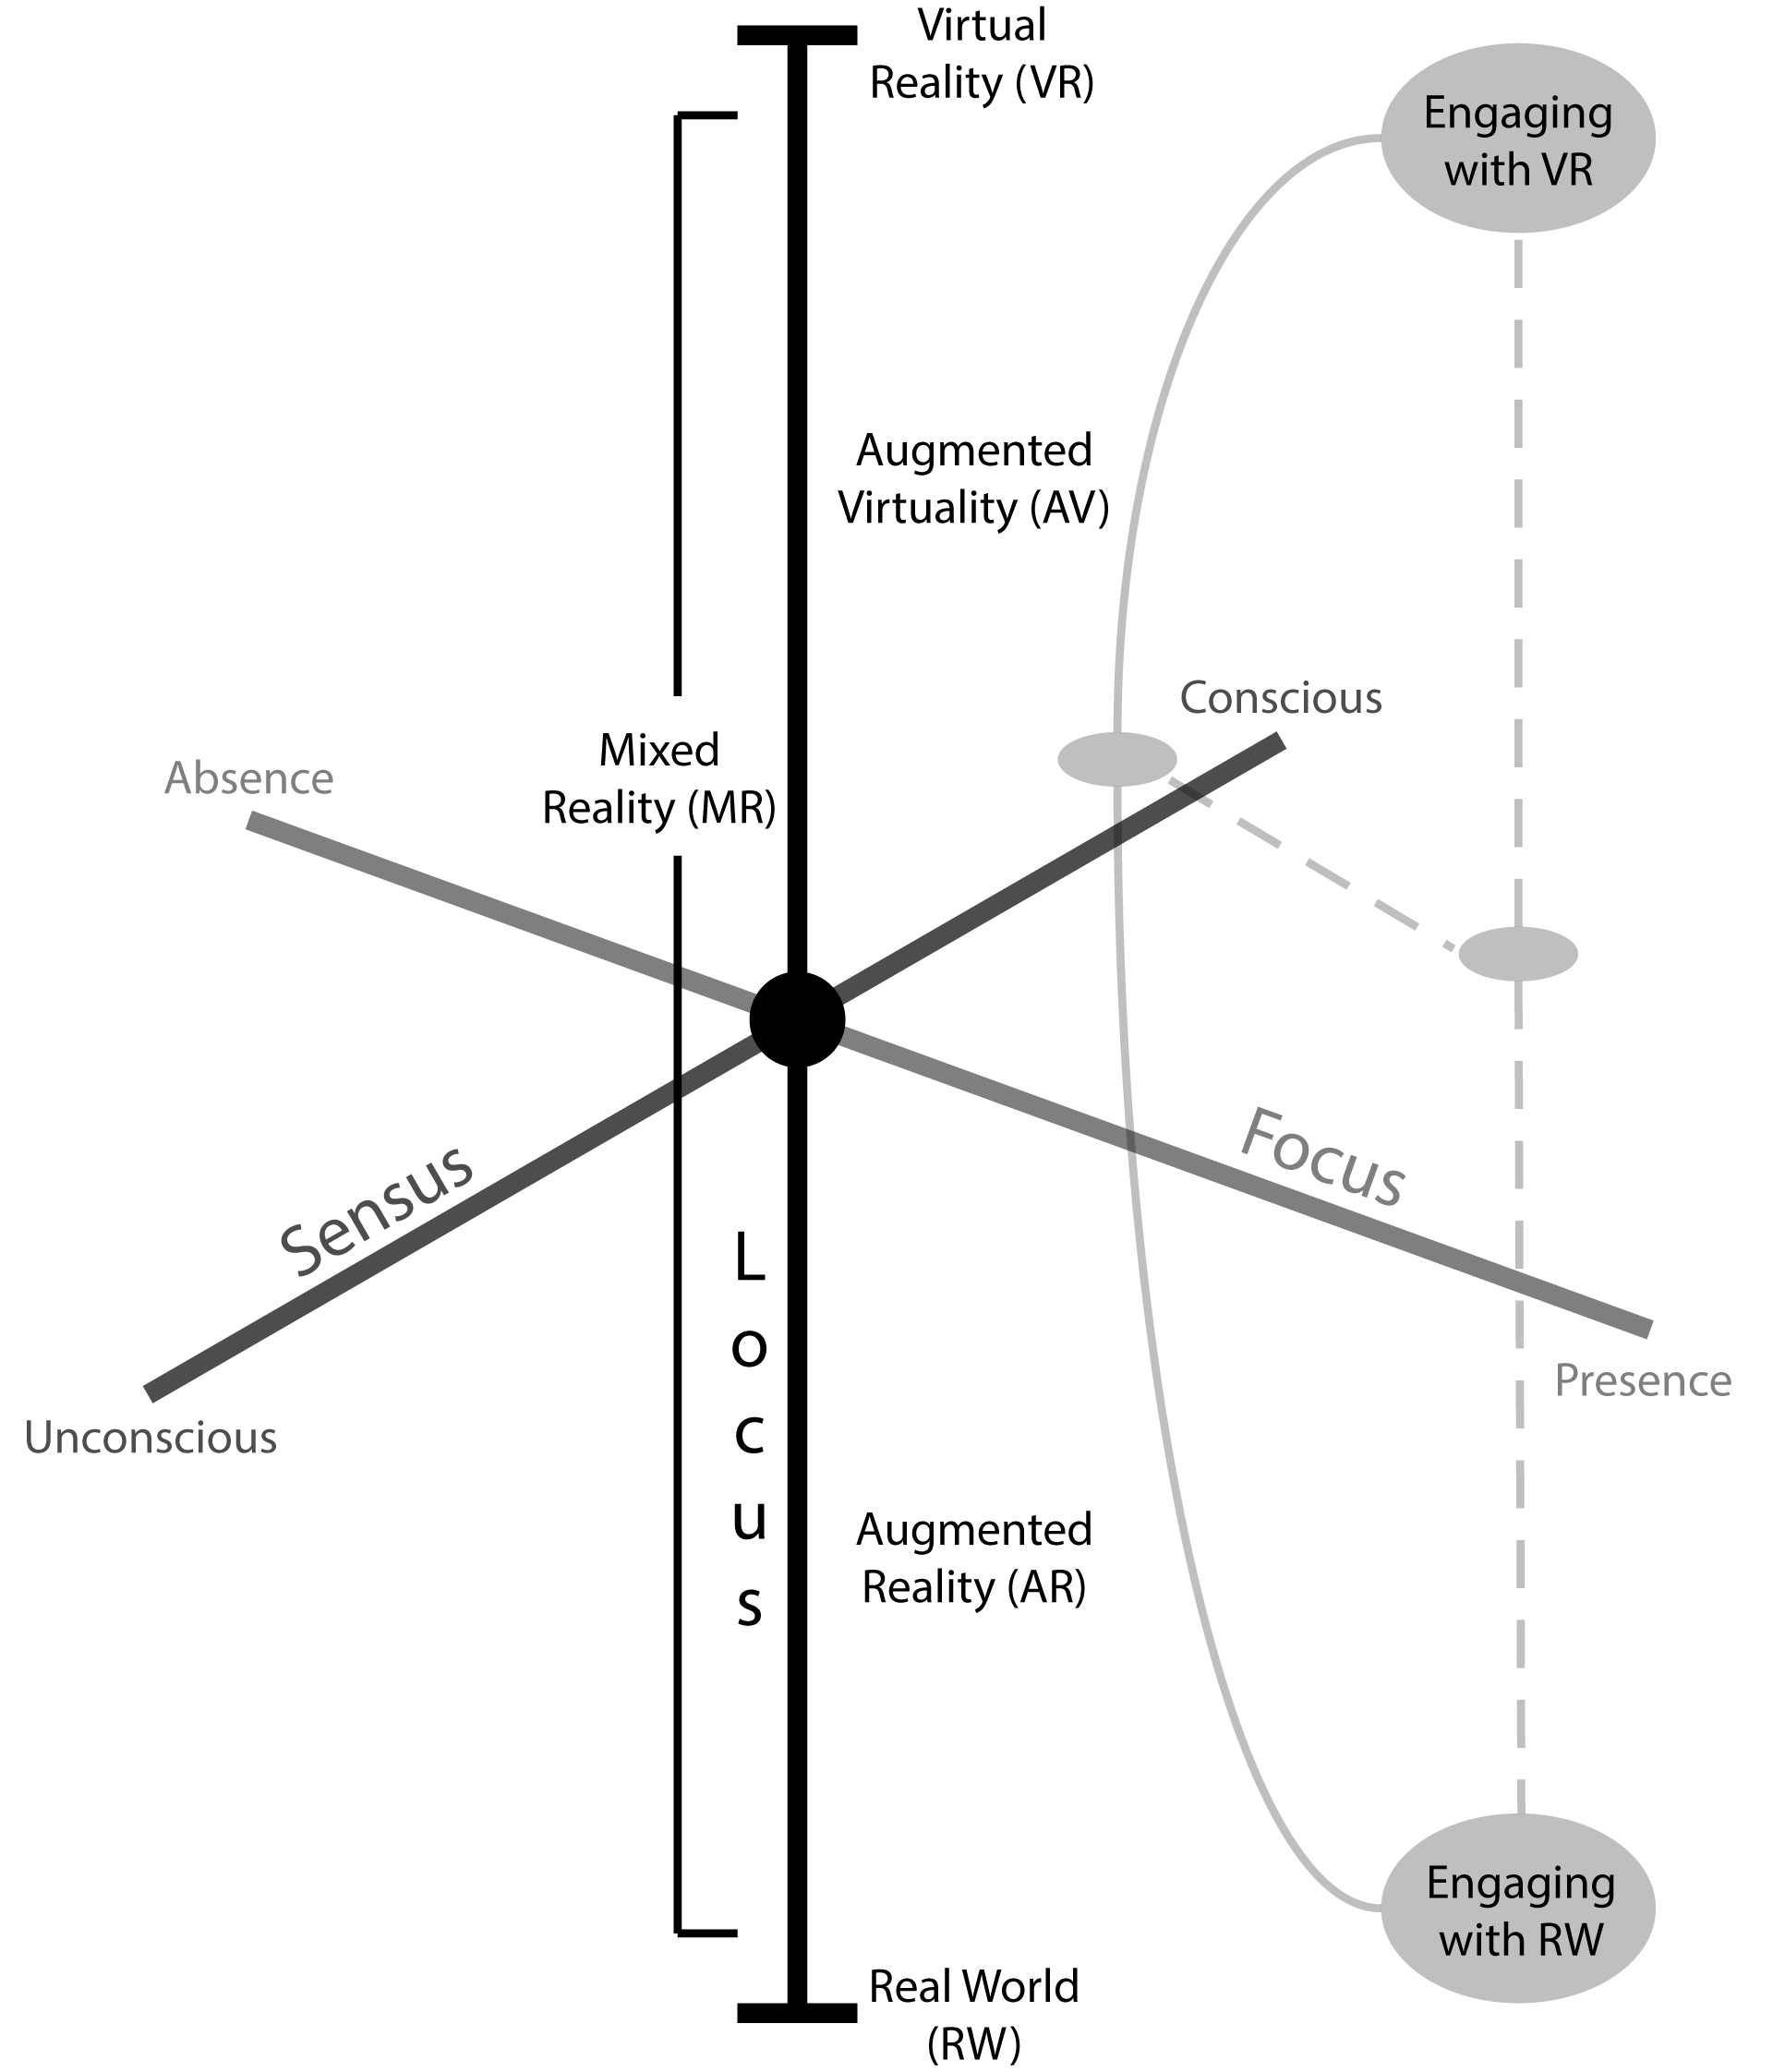
\includegraphics[width=0.7\textwidth]{focus-locus-sensus-with-virtuality-continuum-with-transition-updated.png}
		\caption{Operation of the Mirrorshades platform represented upon the combined model.}
		\label{focus-locus-sensus-with-virtuality-continuum-with-transition}
	\end{center}	
\end{figure}

%=========================================================================================================
%=========================================================================================================

\clearpage


%=========================================================================================================
%=========================================================================================================
%=========================================================================================================
%=========================================================================================================
%=========================================================================================================
%=========================================================================================================
%=========================================================================================================
%=========================================================================================================
%=========================================================================================================
%=========================================================================================================


Users are free to explore and interact with either environment in relative isolation from the other, even if their interactions in one trigger changes in the other, however simultaneous interaction and exploration with both environments has largely remained without systematic investigation.

This is largely because users exploring and interacting with the real environment do not have a convenient manner of also exploring and directly interacting with the virtual environment, as such interaction usually relies upon the use of software run on a desktop or laptop computer which is not conducive to mobile use. Using a laptop computer whilst walking around is far from convenient and using a desktop computer obviously limits the user's interaction with the real environment to that immediately around the location of the  computer and results in a disjoint relationship between their physical position in the real environment and the location of their avatar in the virtual environment when they navigate their avatar away from the respective position of their computer. This situation has been called `the vacancy problem'; an apparent vacancy from one environment whilst engrossed in the other.




%=========================================================================================================
%=========================================================================================================





%=========================================================================================================

Marie Kim et al at The Electronics and Telecommunications Research Institute, Korea, explain the cross reality paradigm well in terms of its principle features

\begin{quote}
\textit{``The important point of X-reality is a paradigm shift from single-directional information flows to bidirectional information flows between two worlds.''}
\end{quote}

and also how it can be employed for simultaneous presence in real and virtual environments

\begin{quote}
\textit{``The differential characteristic of X-reality is that it can augment user's engagement in the experiences of virtual presence and virtual world. Ultimately, it results in the human life span extension from the only real world to both worlds.''}
\end{quote}





Paradiso in IEEE Pervasive, Cross Reality Environments ~\cite{Paradiso2009} \textbf{***check this is the right citation***}

\begin{quote}
\textit{We call the ubiquitous mixed reality environment that comes from the fusion of these two technologies cross-reality. Sensor networks can tunnel dense real-world information into virtual worlds, where this data is interpreted and displayed to dispersed users. Interaction of virtual participants can incarnate into the physical world through a plenitude of diverse displays and actuators. We can envision a user's interface into this environment as an extension of human perception and interaction, augmenting our five senses well beyond the canonical ``here and now'' and redefining the meaning of presence.''}
\end{quote}



\begin{quote}
\textit{``We see cross-reality precipitating when diverse and ubiquitous sensor and actuator networks meet pervasively shared online virtual worlds, where phenomena freely tunnel between real and contrived continua at a multitude of ``wormholes'' opened by densely deployed networked devices, seamlessly adapting the level of immersion to match a variable ecology of available interfaces and user context or preference.''}~\cite{Lifton2009}
\end{quote}



%=========================================================================================================

\section{The Case for Mobile XR}

%ARCHEOGUIDE makes the point that AR is good because users are not isolated/completely immersed in a synthetic world - well Mirrorshades allows uers to more fully immerse themselves in a synthetic world, but without becoming isolated in it (eg without becoming ***vacant*** from the real world)

A XR system that presents the user with visual stimuli from both its constituent environments (RW \& VR) allows that user to engage with both real \& virtual content in a manner that is similar to, but has a number of advantages over, a traditional AR system;

\begin{itemize}
	\item the XR system is less critical of registration (the accurate positioning/alignment) between real \& virtual, as the virtual objects are seen as part of a larger virtual environment instead of being rendered atop a view of the real environment;
	\item the XR system can make use of existing VR content without the overhead of decanting/extracting a subset of the virtual components into an AR framework (e.g. manually selecting which objects within the VR environment are to be displayed over the RW environment);
	\item the use of a complete VR environment allows the virtual content to be more encompassing \& immersive, as presenting a complete VR environment allows total control over lighting, shadows, reflections, particle effects, etc. which would be difficult or impossible for an AR platform to render atop a view of a RW environment.
\end{itemize}

Thus, such a XR platform is well suited to situations in which interaction with both real \& virtual visual stimuli is required \& where one or more of the following hold true;

\begin{itemize}
	\item in lieu of accurate registration between real \& virtual, there is a strong focus on the virtual environment's atmosphere \& immersion~\cite{deamicis:gamebased};
	\item there is existing VR content;
	\item the visual differences between real \& virtual environments are so substantial that an AR system would resort to augment (\&/or diminish~\cite{Mann2002}) almost the whole RW view. While AR \textit{``smears an informational coating over real space''}~\cite{Andersen}, XR presents a complete, discrete virtual environment. AR is beneficial where one wishes the juxtaposition of virtual objects upon what is already present in the RW environment, however VR is better suited to situations where one wishes to present a complete virtual alternative.
\end{itemize}

%=========================================================================================================

% Original literature review from here on

Reviewing the literature on the domain of alternate realities this research finds that there is a gap in the scholarly investigation of simultaneous presence in real and virtual environments and the associated `vacancy problem'. This review proposes that a better understanding of the extension of human presence from only one of the real world or a virtual environment to simultaneous presence in both will permit the introduction of novel systems in a variety of fields in which simultaneous interaction and exploration of both real and virtual environments is possible. Such systems will likely be formed by expansion of research into \textit{cross reality}, an alternate reality comprised of complete real and virtual environments able to mutually reflect and influence each other via sensor/actuator infrastructure, and are likely to be in high demand as progress toward 3D extension of the Web continues.

\section{Conclusions}
We are rapidly approaching a situation in which ubiquitous sensor/actuator infrastructure allows us to access vast amounts of information about any location at any time and additionally to act upon this information and affect these locations. The continuing adoption of fast Internet connections, the increasing ability of commodity hardware including portable devices such as mobile phones and tablets to render complex three-dimensional graphics, and the development of 3D multi-user virtual environments that place an emphasis on notions of community, creation and commerce instead of competitive gaming, all point toward a continuing natural progression toward 3D extension of the Web on a large scale.

It is already common to see people spending substantial amounts of time immersed in the 2D textual/graphical Web whilst simultaneously interacting with the real world around them. This desire to maintain a Web presence whilst simultaneously interacting with the real world is set to remain as interaction with the Web evolves from 2D to 3D. Thus it is prudent to investigate approaches for implementing and applications for exploiting the concept of simultaneous presence in real and virtual 3D environments, whether spatially equivalent or not.

This review has unearthed a plenitude of research on numerous alternate realities, either experienced in isolation from other realities (reality, virtual reality) or by mixing limited amounts of one with another (augmented reality, augmented virtuality) however has discovered a comparative lack of research attention focussed on the concept of simultaneous presence and interaction with two complete environments, one real and the other virtual. Cross reality is the closest existing concept, however the vast majority of the research in this field has used statically located computers to access the virtual environments, preventing users from exploring or interacting with the real environment that is not immediately surrounding them; the true notion of simultaneous presence in real and virtual environments requires freedom of movement and interaction with both environments, perhaps by adopting a manner of interaction with the virtual environment similar to that of the VTW project.

This deficiency of research into simultaneous presence in real and virtual environments warrants addressing with further academic investigation, as it represents a style of interaction that is bound to become commonplace as progress toward 3D extension of the Web continues at an accelerated pace.
